% This is LLNCS.DEM the demonstration file of
% the LaTeX macro package from Springer-Verlag
% for Lecture Notes in Computer Science,
% version 2.4 for LaTeX2e as of 16. April 2010
%
\documentclass{book}
%

\usepackage{makeidx}  % allows for indexgeneration
\usepackage{array}
\usepackage{multirow}
\usepackage{color}
% \usepackage{subfigure}
\usepackage{subcaption}

\usepackage{epsfig}
\usepackage{chngpage}
\usepackage{graphicx}
\usepackage{cite}
\usepackage{arydshln,amssymb,color}
\usepackage[cmex10]{amsmath} 
\usepackage{url}

\usepackage[Algoritmo]{algorithm}

\usepackage{algpseudocode}
\usepackage{programs}
\usepackage{sectsty}
\usepackage[newparttoc]{titlesec}
\usepackage{titletoc}
\usepackage{afterpage}
\usepackage{pdflscape}
\usepackage[utf8]{inputenc}
\usepackage[spanish,es-nodecimaldot]{babel}


\DeclareMathOperator*{\argmin}{argmin}

\graphicspath{{Diagrams/}}

\urldef{\mails}\path|djoroya@gmail.com-address|    
\newcommand{\keywords}[1]{\par\addvspace\baselineskip
\noindent\keywordname\enspace\ignorespaces#1}

\setcounter{secnumdepth}{3}
\setcounter{tocdepth}{3}

%para formatear etiqueta part y su tamaño
%http://tex.stackexchange.com/questions/42526/how-to-remove-page-break-after-part-in-report-book
\titleclass{\part}{top}
%\partfont{\large}
\titleformat{\part}[display]
  {\normalfont\huge\bfseries}{\centering\partname\ \thepart}{20pt}{\large\centering}
%\titlespacing*{\part}{0pt}{50pt}{40pt}
\titlespacing*{\part}{0pt}{0pt}{40pt}

%http://tex.stackexchange.com/questions/54321/how-to-add-spaces-between-items-in-toc
\titlecontents{part}[3pc]{\addvspace{3pc}\filcenter}
  {\sffamily\bfseries\MakeUppercase{\partname}~\thecontentslabel\\*[.2pc]\large}
  {\sffamily\bfseries\large}{}[\addvspace{3pc}]


  \usepackage{geometry}
 \geometry{
 a4paper,
 total={165mm,247mm},
 left=20mm,
 top=20mm,
 }

 \newcommand{\As}{\mathcal{A}}
 \newcommand{\Rs}{\mathcal{R}}
 \newcommand{\Ss}{\mathcal{S}}
 \newcommand{\comment}[1]{[\textcolor{red}{#1}]}



 \usepackage{amsmath}
\numberwithin{equation}{section}
\usepackage{cancel}
\usepackage{bm}


\usepackage{hyperref}
\hypersetup{colorlinks,
%citecolor=blue
}

\usepackage{ntheorem,lipsum}


\theorembodyfont{\upshape}
\newtheorem{thm}{Teorema}[section]
% \newtheorem{lemma}{Lemma}[section]

\newtheorem{defi}{Definición}[section]

\newtheorem{cor}{Colorario}[section]
\newtheorem{obs}{Observación}[section]
\newtheorem{prop}{Proposition}[section]
% \newtheorem{question}{Question}[section]
\newtheorem{example}{Ejemplo}[section]
\newtheorem{problem}{Problema}[section]
\newtheorem{hipo}{Hipotesís}[section]

\newtheorem{db}{Base de datos}[section]

% tombstone like in puthesis
% Proof in boldface like in puthesis

\usepackage[affil-it]{authblk}

\usepackage{smartdiagram}
\usepackage[colorinlistoftodos, spanish, textsize=small]{todonotes}

\usepackage{tikz}
\usetikzlibrary{shapes.geometric, arrows}
\usetikzlibrary{positioning}
\usetikzlibrary{decorations.pathmorphing} % required in the preamble
\usepackage{graphicx}



\usepackage{soul}
 

\begin{document}

%
\frontmatter          % for the preliminaries
%
\pagestyle{plain}  % switches on printing of running heads
%\addtocmark{Hamiltonian Mechanics} % additional mark in the TOC
%
 

\mainmatter              % start of the contributions
%
\title{Sistemas de sistemas de recomendación mediante aprendizaje por refuerzo}

%
% \subtitle{Teoría y algoritmos}
\author{Deyviss Jesús Oroya Villalta}

%\authorrunning{Josu Ceberio et al.} % abbreviated author list (for running head)
 
% \institute{
% Advisor: Roberto Santana Hermida \\
% Intelligent Systems Group,\\ Department of Computer Science and Artificial Intelligence, \\
% University of the Basque Country UPV/EHU,\\
% Paseo Manuel de Lardizabal, 1\\
% Donostia, 20018 Gipuzkoa, Spain\\
% \mails}



\maketitle              % typeset the title of the contribution



%table of content
\tableofcontents
\listoffigures

%\let\cleardoublepage\clearpage

% {\abstract
% Introdución al aprendizaje por refuerzo ...
% }
% {\keywords Proceso de decisión de Markov, Aprendizaje por refuerzo}




\chapter*{Introducción}
\addcontentsline{toc}{chapter}{Introducción}
%% Introducción de sistemas de recomendación

\textcolor{red}{PRESETACION TESIS}


%% Pipeline
%%
%% - Marco Teorico RF
%% - Sistemas de Recomendación
%% - Agrupamiendo de Sistemas de recomendación
%% - 
%
\chapter{Introducción al aprendizaje por refuerzo}
% ¿Que es el aprendizaje por refuerzo?

El aprendizaje por refuerzo es una técnica de aprendizaje automático capaz de resolver problemas de forma dinámica.
Esta técnica se define como un proceso iterativo donde existe un agente capaz de tomar decisiones y un sistema dinámico influenciado por este.
Debido a la interacción entre el agente y el sistema dinámico, el agente  puede controlar el sistema a configuraciones de interés. Estas  configuraciones de interés vienen caracterizadas por una función de coste que es máxima cuando la configuración es alcanzada. 
% 
%
%Por otra parte, el aprendizaje por refuerzo y los problemas clásicos de ontrol óptimo tiene gran similitud. En los problemas de control se define un funcional de coste que depende de valor de acciones que toma el agente y del valor estado que toma el sistema a lo largo de un intervalo temporal. Sin embargo en aprendizaje por refuerzo se añade un grado de complejidad más. Mientras que en los problemas de control óptimo la relación entre las acciones y el estado del sistema es conocido para la resolución del problem, en aprendizaje por refuerzo no lo es. De esta forma, sin conocimiento del sistema el agente debe diseñar estrategicas de control solo a partir de las medidas de la acción, de l estado y de la recompensa obtenida.
%
El aprendizaje por refuerzo utiliza el principio de la programación dinámica para obtener una estrategia de actuación, sin necesidad de conocer la ecuación dinámica del sistema.
\newline

% Introducción de lo que se va a presentar
A lo largo de este capítulo describiremos formalmente el aprendizaje por refuerzo como un proceso de decisión de Markov, enseñando algunos ejemplos. 
%
Luego de esto introduciremos la programación dinámica como método para abordar el problema presentado en el marco de los procesos de decisión de Markov. 
%
Por último, mostraremos algunos algoritmos estándar para abordar este tipo de problemas.

\section{Proceso de decisión de Markov}

Un proceso de decisión de Markov es un proceso dinámico en tiempo discreto y probabilístico capaz de modelizar una gran variedad de procesos. 
%
Este marco matemático es conocido por lo menos desde la decada de 1950, donde en \cite{bellman1957theory} se escribía formalmente por primera vez.

A través de este capítulo usaremos la notación introducida en \cite[cap. 3]{sutton2018reinforcement}. 
 
\begin{defi}[Proceso de decisión de Markov]
Se define un proceso de decisión de Markov como una tupla de cuatro objetos:
\begin{itemize}
    \item Una variable aleatoria $S_t \in \Ss$, que representa el estado en la iteración $t$.
    \item Una variable aleatoria $A_t \in \As$, que representa la acción en la iteración $t$.
    \item Una variable aleatoria $R_t \in \Rs$, que representa la recompensa obtenida en la iteración $t$.
    \item Una distribución de probabilidad: 
    \begin{gather}\label{pdynamics}
        \mathbb{P}(S_{t}= s',R_{t} = r|S_{t-1} = s ,A_{t-1} = a) = p(s',r|s,a)
    \end{gather} 
    Donde a la función $p:\Ss \times \Rs \times \Ss \times \As \rightarrow [0,1]$ será llamada la \textbf{función dinámica} del proceso de decisión de Markov. Esta representa la probabilidad de que estando en el estado $s$ y tomando la acción $a$, obtengamos la recompensa $r$ y transitemos al estado $s'$. 
    \hfill\ensuremath{\square}
\end{itemize}
\end{defi}


\begin{obs}
   Aunque el espacio de recompensas puede ser infinito, a lo largo de este capítulo consideraremos que el espacio de recompensas $\Rs$ es un espacio discreto y finito. Debido a esto siempre podemos sumar en todo el espacio $\Rs$. 
\end{obs} 

Por otro lado, existe otras distribuciones de probabilidad que pueden ser obtenidas de la función dinámica $p(s',r|s,a)$. Estas distribuciones son las distribución de probabilidad de transición y de recompensa.

La distribución de probabilidad de transición $p(s'|s,a)$ se puede obtener como:

\begin{gather}\label{p(s'|s,a)}
    p(s'|s,a) =\sum_{r \in \Rs}  p(s',r|s,a)
\end{gather}

Mientras que  la distribución de probabilidad de recompensa $p(r|s,a)$ se obtiene de la siguiente manera:

\begin{gather}
    p(r|s,a) = \sum_{s' \in \Ss} p(s',r|s,a)
\end{gather}

\begin{obs}
    La distribución de probabilidad de la dinámica $p(s',r|s,a)$, la distribución de probabilidad de transición $p(s'|s,a)$ y la distribución de probabilidad de recompensa $p(r|s,a)$ son funciones distintas aunque utilicemos la misma letra $p$  para referirnos a ellas. Aunque este es un abuso de notación, podemos referirnos a las distintas distribuciones de probabilidad sabiendo que tienen número de argumentos de entrada distintos (véase el cuadro (\ref{DisNot})). 

    \begin{table}[h!]
        \centering
        \begin{tabular}{|c|c|c|}
        \hline
        \textbf{Distribución de probabilidad} &
        \textbf{Función}                      & 
        \textbf{Notación}     \\  \hline
        de la dinámica  &
        $p: \Ss \times \Rs \times \Ss \times \As \rightarrow [0,1]$ &
        $p(s'r|s,a)$ \\ \hline
        de transición   &
        $p: \Ss \times \Ss \times \As \rightarrow [0,1]$ &
        $p(s'|s,a)$ \\ \hline
        de recompensa   &
        $p: \Rs \times \Ss \times \As \rightarrow [0,1]$ &
        $p(r|s,a)$ \\ \hline        
        \end{tabular}
        \caption{Notación de distribuciones de probilidad.}
        \label{DisNot}
        \end{table}
\end{obs}
 
Por otra parte, podemos obtener la recompensa esperada debido a la acción $a$ y estando en el estado $s$ como una función $r: \Ss \times \As \rightarrow \Rs $ tal que:
\begin{gather}\label{r(s,a)}
    r(s,a) = \mathbb{E}[R_t|S_{t-1}=s,A_{t-1}=a] = 
    \sum_{s'\in\Ss} \sum_{r\in \Rs} r \ p(s',r|s,a)
\end{gather}

\begin{obs}
     La letra $r$ se utiliza para denotar  una variable aleatoria asociada a la recompensa, mientras que utilizamos la notación $r(s,a)$ para referiremos a la esperanza de la variable aleatoria $r$ debido a la acción $a$ y estando en el estado $s$. 
\end{obs}


Aunque en la definición formal de un proceso de decisión de Markov es necesario definir la distribución de probabilidad de la dinámica $p(s',r|s,a)$, es habitual definir el proceso de decisión de Markov mediante la distribución de probabilidad de transición $p(s'|s,a)$ y la distribución de probabilidad recompensa $p(r|s,a)$. 
%
Además también es posible definir un proceso de decisión de Markov, mediante la recompensa esperada $r(s,a)$ y la distribución de probabilidad de transición $p(s'|s,a)$. 
%
Estas tres formas de definir los procesos de decisión de Markov son equivalentes, sin embargo dependiendo de la aplicación una es más conveniente que otra (véase el ejemplo \ref{ControlParticula}). 



Con respecto al comportamiento del agente, se define la regla de decisión y la política para su caracterización. Estos objetos nos indican que acciones tomará el agente o como dependen estas acciones del estado.


\begin{defi}[Regla de decisión]
    En el momento de tiempo $t\in \mathbb{N}$ una \textbf{regla de decisión} es una función $\pi_t:\mathcal{S} \rightarrow \As$, que para cada elemento $s \in \mathcal{S}$ asocia $a \in \As$. 
    \hfill\ensuremath{\square}
\end{defi}

\begin{defi}[Política]
Se define como \textbf{política} de un proceso de decisión de Markov como una secuencia de reglas de decisión, $\pi = (\pi_1,\dots,\pi_T)$ que se aplican en un proceso de decisión. Podemos definir un espacio de posibles políticas $\Pi = \As\times \As \times \dots \times \As =\As^T$, tal que $\pi \in \Pi$
\hfill\ensuremath{\square}
\end{defi}

Entonces dadas esta definiciones previas podemos formular cualquier proceso de decisión de Markov. Con el objetivo ejemplificar las definiciones presentadas anteriormente veremos  un ejemplo de proceso de decisión de Markov.
 
\begin{example}[Control de una partícula]\label{ControlParticula}

    Sea el espacio de estados $\Ss = \{ s_1, s_2 ,s_3\}$  y el espacio de acciones $\As = \{\leftarrow \ , \ = \ , \ \rightarrow\}$. 
    %
    Además sea la distribución de probabilidad de transición $p(s',r|s,a)$, donde suponemos que la variable aleatoria recompensa $r$ y la variable aleatoria de estado siguiente $s'$ son independientes. 
    %
    Entonces podemos factorizar la distribución de probabilidad de la dinámica:
    \begin{gather}
        p(s',r|s,a) = p(r|s,a)p(s'|s,a)
    \end{gather}
    En este caso podemos definir la distribución $p(r|s,a)$ y la distribución $p(s'|s,a)$ por separado. Definiremos estas dos distribuciones de forma determinista. Para ello utilizaremos la función delta de Kronecker $\delta$ definida como:
    
    \begin{gather*}
        \delta(x,y) = \begin{cases}
            0 & x \neq y \\
            1 & x  = y
        \end{cases}
    \end{gather*}
    

    En primer lugar, definiremos la distribución de probabilidad de transición $p(s'|s,a)$. Para ello asociaremos cada uno de los estados $\{s_1,s_2,s_3\}$ a los vectores unitarios de $\mathbb{R}^3$: 
    \begin{gather}
        \{s_1,s_2,s_3\} \rightarrow \{(1,0,0),(0,1,0),(0,0,1)\}
    \end{gather}
    Definimos la función $f_s:\Ss \times \As \rightarrow\Ss$ como:
    \begin{gather}
        f_s(s,a) = 
        \delta(a,\leftarrow)\begin{bmatrix}
            1 & 0 & 0  \\
            1 & 0 & 0 \\
            0 & 1 & 0
        \end{bmatrix}  s + 
        \delta(a,=)\begin{bmatrix}
            1 & 0 & 0  \\
            0 & 1 & 0 \\
            0 & 0 & 1
    \end{bmatrix}  s + 
    \delta(a,\rightarrow)\begin{bmatrix}
            0 & 1 & 0  \\
            0 & 0 & 1 \\
            0 & 0 & 1
    \end{bmatrix}  s 
    \end{gather}
    Con ayuda de esta función $f_r(s,a)$ podemos definir la distribución de probabilidad $p(s'|s,a)$ como:
    
    \begin{gather}\label{deltas}
        p(s'|s,a) = \delta(s',f_s(s,a))
    \end{gather}

    En la figura (\ref{graphMDP}) se muestra un representación gráfica de la distribución de probabilidad de transición. Allí podemos ver que está definición simplemente representa una partícula que puede moverse en un recta con tres posiciones y que las acciones que podemos tomar representa un movimiento a la derecha, a la izquierda o quedarnos en la posición en la que nos encontramos. \newline

    En segundo lugar, definiremos la distribución de probabilidad de recompensa $p(r|s,a)$. Para ello definimos la función $f_r:\Ss \times \As \rightarrow \{-2,-1,9,10\}$, como:
    \begin{gather}
        f_r(s,a) = 
        \begin{cases}
            10 - \delta(a,\rightarrow) - \delta(a,\leftarrow) & s = s_2      \\
            -1 - \delta(a,\rightarrow) - \delta(a,\leftarrow) & s \neq s_2
        \end{cases}
    \end{gather}

    Entonces podemos definir la distribución de probabilidad $p(r|s,a)$ como:
    \begin{gather}\label{deltar}
        p(r|s,a) = \delta(r,f_r(s,a)) 
    \end{gather}
    
    Suponemos que el hecho de moverse penaliza en una unidad la recompensa. Además que el sistema alcanza el máximo en la posición $s=s_2$
        

    
    \begin{figure}
        \begin{subfigure}[b]{0.4\textwidth}
            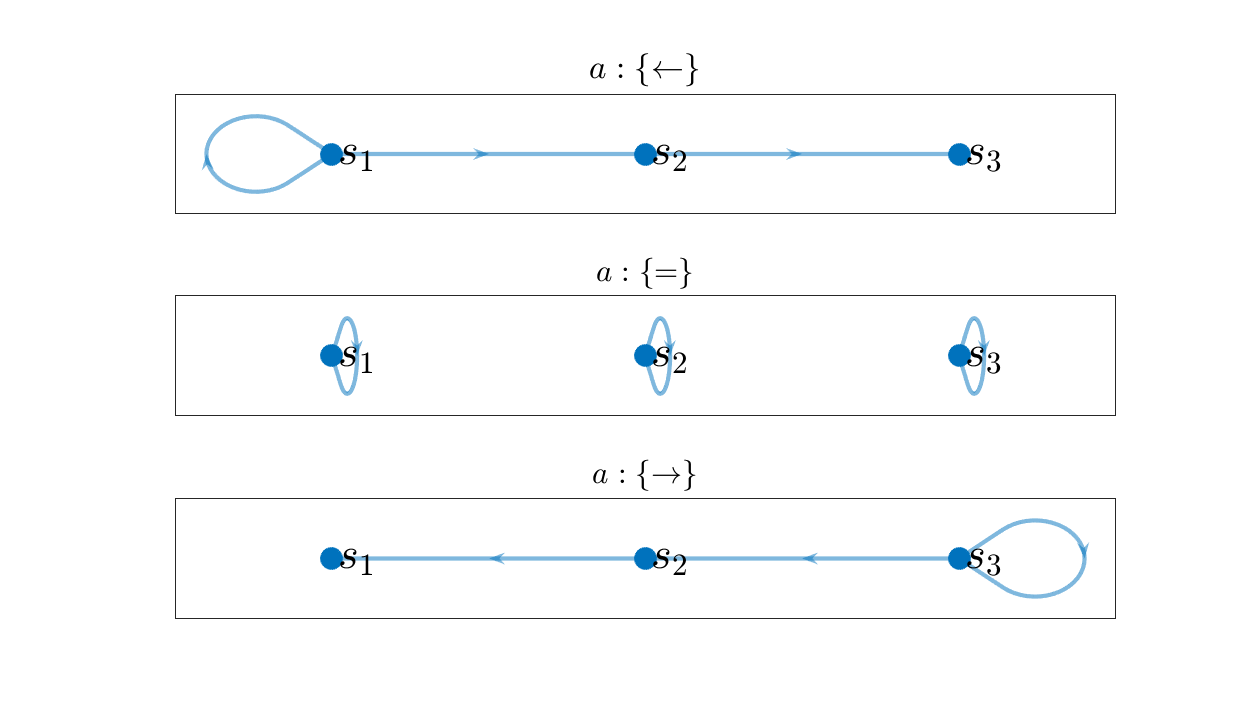
\includegraphics[scale=0.435]{img/particula_estocastica_MDP.eps}
            \caption{Proceso de decisión de Markov.}{\small Para cada posible acción se puede definir una matriz que a su vez se puede representar como un grafo.}
            \label{graphMDP}
        \end{subfigure}
        \hspace{1.75cm}
        \begin{subfigure}[b]{0.4\textwidth}
            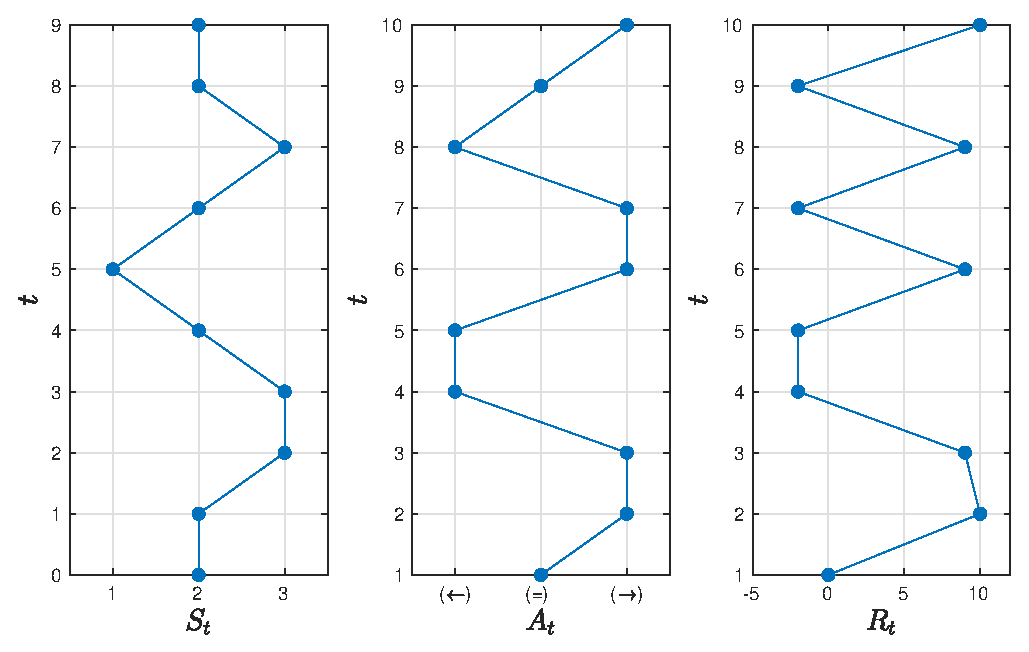
\includegraphics[scale=0.435]{img/MDP_evolution.eps}
            \caption{Evolución del sistema bajo una política.}{\small De una manera intuitiva, el agente actúa en el sistema como si tuviera un mando derecha-izquierda.}
            \label{EvolutionMDP}
        \end{subfigure}   
        \hfill
        \caption{Proceso de desición de Markov para el ejemplo (\ref{ControlParticula}) }
        \label{MDPfig}
    \end{figure}
 


    Por otra parte podemos calcular la recompensa esperada para este sistema:
    \begin{gather}
        r(s,a) = \sum_{r\in \Rs} r \sum_{s'\in\Ss} p(s',r|s,a) =         \sum_{r\in \Rs} r \sum_{s'\in\Ss} p(s'|s,a) p(r|s,a) 
    \end{gather}
    Utilizando las ecuaciones (\ref{deltar}) y(\ref{deltas}):    
    \begin{gather}
        r(s,a) = \sum_{r\in \Rs} r \sum_{s'\in\Ss} \delta(s',f_s(s,a)) \delta(r,f_r(s,a)) = f_r(s,a)  
    \end{gather}
    Asi podemos que que  $r(s,a) = f_r(s,a)$, por lo que en este ejemplo definir la distribución de probabilidad de recompensa $p(r|s,a)$ o la recompensa esperada $r(s,a)$ son equivalentes.
    
    Para concluir, notemos que con la distribución de probabilidad de transición $p(s'|s,a)$ y la distribución de probabilidad de recompensa $p(r|s,a)$, el proceso de desición de Markov del control de una partícula queda completamente caracterizado.

\end{example}

Los conceptos presentados son suficientes para definir correctamente un proceso de decisión de Markov. A partir de estos se puede definir una función de recompensa que nos determinará que tan cerca estamos a la configuración deseada. Este se llama \textbf{retorno esperado} 

\begin{defi}
Se define el \textbf{retorno esperado} a iteración $t$, como la suma de las recompensas desde la iteración $t+1$ hasta la iteración final $T$
\begin{gather}
    G_t = R_{t+1} + \gamma R_{t+2} + \gamma^2 R_{t+3} + \dots =\sum_{\tau= 0}^T \gamma^\tau R_{\tau+t+1}
\end{gather}
Donde $\gamma \in (0,1)$, es llamado el factor de descuento.
\hfill\ensuremath{\square}
\end{defi} 

\begin{obs}
    El factor de descuento $\gamma$ impide que el retorno esperado diverja cuando el horizonte temporal es $T=\infty$, siempre que las recompensas estén acotadas en todo el espacio $\Rs$. Un segundo propósito de este factor es dar más importancia las recompensas obtenidas en un tiempo cercano. 
\end{obs}
\begin{obs}[Recurencia del retorno esperado]
    Es importante notar que cuando el horizonte temporal $T$ es infinito el retorno esperado $G_t$ cumple:
    \begin{gather}\label{Gttt}
        G_t = R_{t+1} + \gamma G_{t+1}
    \end{gather}
\end{obs}

El aprendizaje por refuerzo tiene como objetivo la maximización el retorno esperado $G_t$ con respecto a la política $\pi \in \Pi$. 

\begin{problem}
    Definimos el \textbf{problema de optimización}
    \begin{gather}
              \label{eq:OCP}
            \max_{\pi \in \Pi}\mathbb{E}_\pi\bigg[ \sum_{\tau=0}^T \gamma^{\tau}R_{\tau+1} \bigg| S_0 = s \bigg] = 
            \max_{\pi \in \Pi}\mathbb{E}_\pi\big[G_0\big| S_0 = s\big]
    \end{gather}
    Donde $\mathbb{E}_\pi$ representa la esperanza con respecto a todas las posibles trayectorias en el espacio de estados tomando la política $\pi$. 
\end{problem}
La solución a este problema también tiene un carácter especial, por que lo definiremos.

\begin{defi}
    Definimos la \textbf{política óptima}, $\pi_*$ como:
    \begin{gather}
        \pi_* \in \arg \max_{\pi \in \Pi}\mathbb{E}_{\pi}\big[G_0| S_0 = s\big]  
    \end{gather}
\hfill\ensuremath{\square}
\end{defi}

Entonces un proceso de decisión de Markov en síntesis consiste maximizar el retorno esperado $G_t$ conrespecto a la  política $\pi \in \Pi$ y sujeto a la distribución de probabilidad de la dinámica $p(s',r|s,a)$.
\section{Programación dinámica}

La programación dinámica es una metodología de optimización, desarrollada en \cite{bellman1954theory}. Aunque en un principio la programación dinámica fue formulada en sistemas discretos deterministas su generalización a procesos probabilísticos fue realizada poco después de su creación en \cite{bellman1957theory}. 


\subsection{Funciones valor estado ($v^\pi$)}

Las funciones valor son la base de la programación dinámica, sus leyes de recurencia nos permiten construir algoritmos en el marco del aprendizaje por refuerzo. A continuación las definiremos.

\begin{defi}[Función valor de estado]\label{defi:valorstado}
    Definición la \textbf{función valor de estado} como una función, $v^\pi:\Ss \rightarrow \mathbb{R}$:
    \begin{gather}
        v^\pi(s) = \mathbb{E}_\pi\big[\sum_{t=0}^\infty \gamma^\tau R_{{\tau+1}}|S_0=s\big]=\mathbb{E}_\pi[G_t|S_t = s]
    \end{gather}
    Donde hemos tomado el horizonte temporal, $T=\infty$.
    \hfill\ensuremath{\square}
\end{defi}


\begin{obs}
    En este documento tomaremos la definición \ref{defi:valorstado} como la definición de función valor de estado, tomando $T=\infty$. Estos problemas  son llamados procesos de decisión de Markov con horizonte infinito. Sin embargo, el horizonte temporal $T$ puede ser finito aunque requiere una definición ligeramente distinta. Puede verse más definiciones en \cite{LAZARIC}.
\end{obs}

Otra pieza fundamental en la programación dinámica es la función valor de estado óptima.

\begin{defi}[Función valor de estado óptima]
    Definimos la \textbf{función valor de estado óptima} como:
    \begin{gather}\label{valorestadoopt}
        v_*(s) = \max_{\pi\in \Pi} v^\pi(s)
    \end{gather}
    Esta función tiene  una clara interpretación en el proceso de decisión de Markov. Esta es la solución del problema de optimización (\ref{eq:OCP}) para una condición inicial $S_0=s$.
    \hfill\ensuremath{\square}
\end{defi}

Si descomponemos $G_t$ utilizando la ecuación (\ref{Gttt}), en la ecuación (\ref{defi:valorstado})

\begin{gather}
    v^\pi(s) = \mathbb{E}_\pi[G_t|S_t = s] = \mathbb{E}_\pi[R_{t+1} + \gamma G_{t+1}|S_t = s]
\end{gather}
Deshaciendo la sumatoria de la esperanza en el primer paso, obetenemos:
\begin{gather}
    v^\pi(s) = \sum_{s',r} p(s',r|s,\pi(s)) \big[r + \gamma \underbrace{\mathbb{E}_\pi[G_{t+1}|S_t = s']}_{v^\pi(s')}\big]
\end{gather}

Y con ello obetenemos la ecuación de Bellman para la función valor de estado.

\begin{cor}[Ecuación de Bellman]
    Entonces la función valor de estado $v^\pi(s)$ cumple la siguiente ecuación:
    \begin{gather}\label{BellmanEquation}
        v^\pi(s) =  \sum_{s',r}p(s',r|s,\pi(s))\bigg[r + \gamma v^\pi(s')\bigg] \\
        \forall s \in \Ss \ , \ \forall t \in \{1,\dots,T\} \notag
    \end{gather}
\end{cor}

Utilizando las ecuaciones (\ref{r(s,a)}) y (\ref{p(s'|s,a)}) podemos re-escribir la expresión anterior de la siguiente manera:

\begin{gather}\label{BellmanEquation}
    v^\pi(s) =  r(s,\pi(s)) + \gamma \sum_{s'}p(s'|s,\pi(s)) v^\pi(s')
\end{gather}

Tomando la definición del la función de estado óptima (\ref{valorestadoopt}) y la expresión anterior:

\begin{gather}
    v_*(s) = \max_{\pi \in \Pi } v^\pi(s) = \max_{\pi \in \Pi } \bigg[ r(s,\pi(s)) + \gamma \sum_{s'}p(s'|s,\pi(s)) v^\pi(s') \bigg]
\end{gather}

Podemos obtener la ecuación de Bellman para la función valor de estado óptima.
\begin{cor}[Ecuación de Bellman óptima]
    Entonces la función valor de estado óptima $v_*(s)$ cumple la siguiente ecuación:
    \begin{gather}\label{BellmanEquationOptimo}
        v_*(s) = \max_{a'} \bigg[ r(s,a') + \gamma \sum_{s'}p(s'|s,a') v_*(s') \bigg]
    \end{gather}
\end{cor}


Esta espresión nos permite recuperar la política óptima tomando el argumento de la maximización anterior:

\begin{gather}
    \pi_*(s) = \arg \max_{a'} \bigg[ r(s,a') + \gamma \sum_{s'}p(s'|s,a') v_*(s')
        \bigg]
\end{gather}

Entonces, podemos obtener las reglas de decisión $\pi_*(s)$ si conocemos la función valor $v_*(s) \ \ \forall s \in \Ss$.\newline

\subsection{Función valor de estado-accion ($q^\pi$)}

En la programación dinámica se define otras dos funciones muy útilies y en ocasiones más conveniente que la función valor de estado. Estas son llamadas la función valor estado-acción y la función valor de estado-acción óptima.

\begin{defi}[Función valor de estado-acción]
    Definimos la función valor de estado-acción como una función, $q^\pi: \Ss \times \As \rightarrow \mathbb{R}$ tal que:
    \begin{gather}
        q^\pi(s,a) = \mathbb{E}_\pi[G_t|S_t = s,A_t=a]
    \end{gather}
    Esta función es similar a la función valor de estado pero con un grado de libertad adicional a la hora de elegir la primera acción. Las sucesivas acciones vienen dada por la política $\pi$.
    \hfill\ensuremath{\square}
\end{defi}


\begin{defi}[Función valor de estado-acción óptima]
    Definimos la función valor de estado-acción óptima como una función, $q_*: \Ss \times \As \rightarrow \mathbb{R}$ tal que:
    \begin{gather}\label{qopt}
        q_*(s,a) = \max_{\pi \in \Pi} q^\pi(s,a)
    \end{gather}
    La función de valor estado-acción óptima tiene una interpresación en el proceso de decisión de Markov. Esta es la solución del problema de optimización (\ref{eq:OCP}) para una condición inicial $S_0=s$ y tomando la primera acción  $A_0=a$.
    \hfill\ensuremath{\square}
\end{defi}


Encontraremos la relación entre $v_*(s)$ y $q_*(s)$, con el fin de definir la manera en la que encontramos la política óptima a partir de $q_*(s)$. \newline


Utilizamos  la recurencia del retorno esperado $G_t$ 
\begin{gather}
    q^\pi(s,a) = \mathbb{E}_\pi[G_t|S_t = s,A_t=a] =
  \mathbb{E}_\pi[R_{t+1} + \gamma G_{t+1} |S_t = s,A_t=a] 
\end{gather}

luego deshacemos el primer sumatorio de la esperanza $E_\pi$:

\begin{gather}
    q^\pi(s,a) = 
   \sum_{s',r} p(s',r|s,a) \bigg[ r + \gamma \underbrace{\mathbb{E}_\pi[ G_{t+1} |S_t = s']}_{v^\pi(s)} \bigg]
\end{gather}


Entonces obtenemos una relación directa entre la función valor estado $v^\pi(s)$ y la función valor estado-acción $q^\pi(s)$:


\begin{gather}\label{qv}
    q^\pi(s,a) =  r(s,a) + \gamma \sum_{s'}p(s'|s,a) v^\pi(s')
\end{gather}

Ahora utilizamos (\ref{qopt}) en (\ref{qv}):

\begin{gather}
    q_*(s,a) = \max_{\pi \in \Pi} \bigg[ r(s,a) + \gamma \sum_{s'}p(s'|s,a) v^\pi(s') \bigg]
\end{gather}

Dado que el término $r(s,a)$ no depende de la política aplicada podemos extraer  de la maximización:
\begin{gather}
    q_*(s,a) =   r(s,a) +  \gamma \sum_{s'}  p(s'|s,a) \max_{\pi \in \Pi}  v^\pi(s')
\end{gather}
Por otra parte, deberemos notar que  la maximización la función $v^\pi(s')$ sobre todas las política $\pi \in \Pi$ es la definición de función valor óptima. Por lo que obtenemos una relación entre la función valor de estado óptima $v_*(s)$ y la función valor de estado-acción $q_*(s,a)$:
\begin{gather}\label{qoptvopt2}
    q_*(s,a) =   r(s,a) +  \gamma \sum_{s'}  p(s'|s,a)v_*(s')
\end{gather}

El lado derecho de la expresión anterior es exactamente le término que se maximiza en la ecuación de Bellman (\ref{BellmanEquationOptimo}). Entonces si remplazamos $q_*(s,a)$ en la ecuación de Bellman obtenemos la relación entre $q_*(s)$ y $v_*(s)$:
\begin{cor}[Relación entre funciones valor óptimas]
    Podemos obtener $v_*(s)$ a partir de $q_*(s,a)$ de la siguiente manera:
    \begin{gather}\label{voptqopt}
        v_*(s) =  \max_{a'\in \As} q_*(s,a')
    \end{gather} 
\end{cor}

Por último, utilizando (\ref{voptqopt}) y (\ref{qoptvopt2}) obtenemos  la ecuación de Bellman para la función valor de estado-acción:
\begin{cor}[Ecuación de Bellman estado-acción óptima]
    \begin{gather}
        q_*(s,a) = r(s,a) +  \gamma \sum_{s'}  p(s'|s,a) \max_{a'\in \As}q_*(s',a')
    \end{gather}
\end{cor}


Estas leyes de recurrencia nos permitiran encontrar la función valor mediante la expresión (\ref{voptqopt}) y mediante esta la política óptima $\pi^*$.


%%%%%%%%%%%%%%%%%%%%%%%%%%%%%%%%%%%%%%%%%%%%%%%%%%%%%%%%%%%%%
%%%%%%%%%%%%%%%%%%%%%%%%%%%%%%%%%%%%%%%%%%%%%%%%%%%%%%%%%%%%%

\subsection{Operadores de Bellman (OB)}

Los operadores de Bellman son una herramienta necesaria para comprender los algoritmos básicos de aprendizaje por refuerzo. Estos nos proveen teormeas fundamentales que nos aseguran la convergende de los algoritmos. Para ello seguiremos el discruso seguido en \cite{LAZARIC}. \newline

Denotaremos con la letra $N$ para representa la cardinalidad del espacio de estados $\Ss$.


% \begin{defi}[OB de estado]
%     Dado un un espacio vectorial $\mathbb{R}^N$ podemos definir el operador de Bellman $\mathcal{T}^\pi:\mathbb{R}^N \rightarrow \mathbb{R}^N$ como:
%     \begin{gather}
%         \mathcal{T}^\pi \mathcal{V}(s) = r(s,\pi(s)) + \gamma \sum_{s' \in \Ss} p(s'|s,\pi(s)) \mathcal{V}(s')
%     \end{gather}
%     \hfill\ensuremath{\square}
% \end{defi}

\begin{defi}[OB de estado óptimo]
    Dado un un espacio vectorial $\mathbb{R}^N$ podemos definir el operador de Bellman $\mathcal{T}:\mathbb{R}^N \rightarrow \mathbb{R}^N$ como:
    \begin{gather}
        \mathcal{T} \mathcal{V}(s) = \max_{a\in\As} \bigg[ r(s,a) + \gamma \sum_{s' \in \Ss} p(s'|s,a) \mathcal{V}(s') \bigg]
    \end{gather}
    \hfill\ensuremath{\square}
\end{defi}


Es fácil ver que $V^\pi$ es punto fijo del operador $\mathcal{T}^\pi$, es decir que al aplicar el operador $\mathcal{T}^\pi$ al vector $V^\pi$ obtenemos otra vez gracias a que $V^\pi$ cumple la ecuación de Bellman (\ref{BellmanEquation}). De la misma manera, $V^* $ es punto fijo del operador $\mathcal{T}$ debido a que cumple la ecuación de Bellman (\ref{BellmanEquationOptimo}).


\begin{thm}[Punto Fijo de Banach \cite{banach1922operations}]
    Dado un espacio vectorial $\mathcal{E}$ equipado con una norma $||.||$ y un operador contractivo $\mathcal{O}:\mathcal{E} \rightarrow \mathcal{E}$. Entonces existe un único punto fijo. Además empezando desde cualquier punto del espacio $v \in \mathcal{E}$ la sucesión:
    \begin{gather}
        \{ v,\mathcal{O}(v) \ , \ \mathcal{O}(\mathcal{O}(v)) \ , \ \mathcal{O}(\mathcal{O}(\mathcal{O}(v))) \ , \ ... \}
    \end{gather}
    converge al punto fijo.
    \hfill\ensuremath{\blacksquare}

\end{thm}

%Los operadores $\mathcal{T}_v$ y $\mathcal{T}_v^\pi$ cumple con contracción en la norma $L_\infty$. Es decir, para todo $\mathcal{V}_1,\mathcal{V}_2 \in \mathbb{R}^N$ , si $\mathcal{V}_1 \leq \mathcal{V}_2$

El $\mathcal{T}_v$ cumple con la contracción en la norma $L_\infty$. Es decir, para todo $\mathcal{V}_1,\mathcal{V}_2 \in \mathbb{R}^N$ , si $\mathcal{V}_1 \leq \mathcal{V}_2$


\begin{gather}
%    || \mathcal{T}_v^\pi \mathcal{V}_1  - \mathcal{T}_v^\pi \mathcal{V}_2||_\infty \leq \gamma || \mathcal{V}_1 - \mathcal{V}_2||_\infty \\
    || \mathcal{T}_v\mathcal{V}_1  - \mathcal{T}_v \mathcal{V}_2||_\infty \leq \gamma || \mathcal{V}_1 - \mathcal{V}_2||_\infty
\end{gather}

% Por lo tanto debido al teorema de punto fijo de Banach, empezando en cualquier estimación inicial de la función valor de estado $\mathcal{V}_0$, la aplicación sucesivas del operador de Bellman nos conduce inevitablemente al punto fijo del operador. En el caso de operador de Bellman $\mathcal{T}^\pi_v$ nos conduce a $v^\pi$, mientras que en el caso del operador de Bellman óptimo $\mathcal{T}_v$ nos conduce a $v_*$. \newline

Por lo tanto debido al teorema de punto fijo de Banach, empezando en cualquier estimación inicial de la función valor de estado $\mathcal{V}_0$, la aplicación sucesivas del operador de Bellman nos conduce inevitablemente al punto fijo del operador. \newline


De la misma manera se puede definir los operadores de Bellman para la función valor de estado-acción $Q(s,a)$. Para ello denotaremos $M$ como la cardinalidad del espacio de acciones.

% \begin{defi}[OB de estado-acción]

%     Dado un un espacio vectorial $\mathbb{R}^{N\times M}$  podemos definir el operador de Bellman $\mathcal{T}^\pi_q:\mathbb{R}^{N\times M} \rightarrow \mathbb{R}^{N \times M}$ como:
%     \begin{gather}
%         \mathcal{T}^\pi_q \mathcal{Q}(s,a) = r(s,a) + \gamma \sum_{s' \in \Ss} p(s'|s,a) \mathcal{Q}(s',\pi(s'))
%     \end{gather}
% \end{defi}

\begin{defi}[OB de estado-acción óptimo]
    Dado un un espacio vectorial $\mathbb{R}^{N\times M}$ podemos definir el operador de Bellman $\mathcal{T}_q:\mathbb{R}^{N\times M} \rightarrow \mathbb{R}^{N\times M}$ como:
    \begin{gather}
        \mathcal{T}_q \mathcal{Q}(s,a) =  r(s,a) + \gamma \sum_{s' \in \Ss} p(s'|s,a) \max_{a'\in\As} \mathcal{Q}(s',a')
    \end{gather}
\end{defi}

Estos dos operadores tienen propiedades análogas a OB que nos permiten decir que mediante la sucesivas aplicaciones del operador $\mathcal{T}_q$ para cualquier vector $\mathcal{Q}(s,a)$ terminaremos encontrando $q^*(s,a)$



\section{Algoritmos de aprendizaje por refuerzo}

Definido ya los operadores de Bellman somos capaces de entender algunos algoritmos de aprendizaje por refuerzo basado en el teorema de punto fijo, además elementos de los métodos de montecarlo. Presentaremos tres alogirmtos: \emph{Value Iteration}, \emph{Q-Iteration} y \emph{Q-learning}.

\subsection*{Value Iteration}
Gracias a que el operador de Bellman de estado $\mathcal{T}_v$ cumpla el teorema de punto fijo de Banach da lugar al algoritmo llamado \emph{Value Iteration}\cite[cap. 4.4]{sutton2018reinforcement}. Este algoritmo requiere aplicar el operador de Bellman para para cada uno de los estados del sistema en cada iteración del algoritmo hasta que la variación de la función valor obtenida sea pequeña con respecto a la iteración anterior (\textit{véase el algoritmo }\ref{ValueIteration}). 


\begin{algorithm}[!ht]
    \caption{\emph{Value Iteration}}\label{ValueIteration}
    \begin{algorithmic}[1]
        \Procedure{Value-Iteration}{$\mathcal{V}^*,tol$}
        \State $k \gets 0$
        \State $\mathcal{V}_k\gets \mathcal{V}^*$
        \While{$error\leq tol$}
            \State $k \gets k + 1$
            \For{$\forall s \in \Ss$}
                \State $\mathcal{V}_k(s)\gets \mathcal{T}_v\mathcal{V}_{k-1}(s)$
            \EndFor
            \State $error \gets || \mathcal{V}_k - \mathcal{V}_{k-1}||_\infty$
        \EndWhile
        \State $\displaystyle \pi_k^*(s) = \arg \max_{a'\in \As} \bigg[ r(s,a') + \gamma \sum_{s'}p(s'|s,a') v_*(s')
        \bigg]$
        \State \textbf{return}: [$\mathcal{V}_k(s)$,$\pi_k^*(s)$]
        \EndProcedure
    \end{algorithmic}
\end{algorithm}



\subsection*{\emph{Q-Iteration}}

De la misma manera que función valor de estado óptima $v_*(a)$, que la función valor estado-acción óptima $q_*(s,a)$ cumpla el teorema de punto fijo de Banach nos permite realizar el mismo procedimiento utilizado en el algoritmo anterior (\emph{véase el algoritmo }\ref{QIteration}). 



\begin{algorithm}[!ht]
    \caption{\emph{Q-Iteration}}\label{QIteration}
    \begin{algorithmic}[1]
        \Procedure{Q-Iteration}{$\mathcal{Q}^*,tol$}
        \State $k \gets 0$
        \State $\mathcal{Q}_k\gets \mathcal{Q}^*$
        \While{$error\leq tol$}
            \State $k \gets k + 1$
            \For{$\forall (s,a) \in \Ss \times \As $}
                \State $\mathcal{Q}_k(s,a) \gets \mathcal{T}_q \mathcal{Q}_{k-1}(s,a)$
            \EndFor
            \State $error \gets || \mathcal{Q}_k - \mathcal{Q}_{k-1}||_\infty$
        \EndWhile
        \State $ \displaystyle \mathcal{V}_k(s) = \max_{a\in \As} Q_k(s,a)$
        \State $ \displaystyle \pi_k^*(s) = \arg \max_{a\in \As} Q_k(s,a)$
        \State \textbf{return}: ($\mathcal{Q}_k(s,a)$ , $\mathcal{V}_k(s)$ , $\pi_k^*(s)$)
        \EndProcedure
    \end{algorithmic}
\end{algorithm}



\subsection*{\emph{Q-learning}}


                                               
El algoritmo de \emph{Q-learning} (\emph{véase algoritmo }\ref{Qlearning}) pretende encontrar una política óptima a través de un proceso a tiempo real y sin conocimiento de la dinámica del sistema. Este utiliza medidas en el estado siguiente $s_{t+1}$ y la recompensa obtenida $r_t$ debido a la acción $a_t$ que tomemos. Si empezamos en un estado inicial $s_0 = s$ y una estimación inicial de la función valor estado-acción $\mathcal{Q}^*$,  podemos elegir la acción a tomar en cada iteración de tiempo mediante esta estimación y medir la recompensa obtenida y el estado al que se ha transitado. Con ayuda de estas medidas podemos mejorar la estimación de la función valor estado-acción.

Para elegir la acción a tomar en cada momento se utiliza una estimación del la función valor de estado-acción $\mathcal{Q}_t$. La acción a tomar se escoge según la siguiente expresión:

\begin{gather}
      a_t \leftarrow \arg \max_{a'\in \As} [\mathcal{Q}_t(s_t,a') ]
\end{gather}

Debido a que la función de valor de estado-acción es aproximada se toman en ciertas iteraciones una acción aleatoria con una pequeña probabilidad $\epsilon$, que evita caer en minimos local. 


Luego se puede actualizar la estimación de la función de valor estado acción mediante la expresión:

\begin{gather}
    \displaystyle \mathcal{Q}(s_t,a_t) \gets    \underbrace{\big[ r(s_t,a_t) + \gamma \max_{a'\in \As}\mathcal{Q}(s_{t+1},a') \big]}_{\approx\mathcal{T}_q \mathcal{Q}(s_t,a_t)}
\end{gather}

En principio deberiamos actualizar la función valor de estado-acción mediante la aplicación directa del operador $\mathcal{T}_q$, sin embargo esto requiere que conozcamos la distribución de probabilidad de transisicón $p(s'|s,a)$. Esto se solventa con la evaluación repetida de $r$ y $s'$ para una acción $a$. Entonces se realizar una media ponderada de los valores obtenidos para $Q(s,a)$. Esto se expresa de forma matemática como:

\begin{gather}
    \displaystyle \mathcal{Q}(s_t,a_t) \gets  (1-\alpha)\mathcal{Q}(s_t,a_t)  + \alpha \bigg[ r(s_t,a_t) + \gamma \max_{a'\in \As}\mathcal{Q}(s_{t+1},a') \bigg]
\end{gather}

Esto nos permite obtener una función valor de estado-acción aproximada que va mejorando a tiempo real y que permite actuar bajo una política desde el primer instante de tiempo.
\begin{algorithm}[!ht]
    \caption{\emph{Q learning}}\label{Qlearning}
    \begin{algorithmic}[1]
        \Procedure{Q-learning}{$\mathcal{Q}^{*},s_0,tol,\alpha,\epsilon$}
        \State $k \gets 0$
        \State $\mathcal{Q} \gets \mathcal{Q}^{*}$
        \While{$error\leq tol$}
            \State $t \gets t + 1$
            \If{$\epsilon > rand$}
                \State $a_t \leftarrow$ acción aleatoria
            \Else
                \State $\displaystyle a_t \leftarrow \arg \max_{a'\in \As} [\mathcal{Q}_t(s_t,a') ]$
            \EndIf
            \State Actuar con $a_t$ y medir $r_{t}$ y $s_{t+1}$
            \State $\displaystyle \mathcal{Q}(s_t,a_t) \gets (1-\alpha)\mathcal{Q}(s_t,a_t) +  
            \big[ r(s_t,a_t) + \gamma \max_{a'\in \As}\mathcal{Q}(s_{t+1},a') \big]$
        \EndWhile
        \State \textbf{return} $\{a_t\}_{t>0}$
        \EndProcedure
    \end{algorithmic}
\end{algorithm}



\begin{example}[Movimiento de una partícula en un potencial]\label{ParticulaPotencial}

    Presentamos un problema de física clásica en el que existe una partícula en un  potencial. El potencial elegido tiene la forma presentada en la figura \ref{fig:potencial}. Este sistema queda caraterizado mediante la posición $x$ y velocidad $v$ en un instante de tiempo dado. Definiremos el problema dentro de una región acotada: 
    \begin{gather}
        x \in [-6,6] \ \ \  v \in [-6,6] 
    \end{gather}
    Por otra parte, debido a que la formulación presentada esta en tiempo discreto, para resolver este problema necesitamos un esquema numérico que nos permita convertir la variable continua $t$ a una variable discreta. Elegiremos el esquema de euler para obtener el sistema dinámico discreto.
    \begin{gather}
        \frac{d}{dt}\begin{bmatrix}
            x(t) \\ v(t)
        \end{bmatrix} = f(x(t),v(t),a(t))
    \end{gather}
    \begin{gather}
        \underbrace{
            \frac{d}{dt}\begin{bmatrix}
                x(t) \\ v(t)
            \end{bmatrix} =
            \begin{bmatrix}
                v(t) \\ -\vec{\nabla}P(x(t))  - \frac{1}{2}x(t) + a(t)
            \end{bmatrix}}_{Tiempo \ continuo}
        \ \Longrightarrow \
        \underbrace{
            \begin{bmatrix}
                x_{t+1} \\ v_{t+1}
            \end{bmatrix} =
            \begin{bmatrix}
                x_t +\Delta t  \ v_t \\
                v_t +\Delta t  \ [-\vec{\nabla}P(x_t)  - \frac{1}{2}x_t + a_t]
            \end{bmatrix}}_{Tiempo \ discreto}
    \end{gather}
    Donde se ha tomando como tamaño de paso $\Delta t = 0.0725$.\newline

    Además se ha discretizado el espacio de estados $\Ss$ y el de acciones $\As$ de la siguiente manera: 
    \begin{itemize}
        \item $\Ss = \underbrace{\{-6.0000 , -5.9195 , \dots, 5.9195  ,  6.0000\}}_{150 \ puntos \ en \ x}\times \underbrace{\{-6.0000 , -5.9195 , \dots, 5.9195  ,  6.0000\}}_{150 \ puntos \ en \ v}$
        \item $\As = \{ -20 ,  -10  ,   0  ,  10   , 20\}$
    \end{itemize}

    Entonces definimos la recompensa esperada como:
    \begin{gather}
        r(s,a) = r([x,v],a) =  100 \exp(-(x^2+v^2)/0.5^2)
    \end{gather}

    Dado en este caso el sistema es determinista, por lo que el operador de Bellman se puede escribir como:

    \begin{gather}
        \mathcal{T}\mathcal{V}(s) = 100 \exp(-(x^2+v^2)/0.5^2) + \max_{a\in \As} \big[   \mathcal{V}(f(s,a))\big]
    \end{gather}
 
    Utilizaremos el algoritmo \emph{Q-Iteration} y el algoritmo \emph{Q-learning} para resolver el problema planteado. Además, con el fin de comparar los algoritmos de aprendizaje por refuerzo con metodologías que tienen en cuenta el conocimiento de la dinámica del sistema, resolveremos el siguiente problema de control óptimo:
    
    \begin{gather}
        \min_{a \in \mathbb{R}} \int_0^\infty (|| s(t)||^2  + ||a(t)||^2 )dt  \\
        sujeto \ a: \notag \\
        \dot{s} = As(t) + Bu(t) \notag
    \end{gather}
    Donde $A$ y $B$ son los jacobiandos de $f$ con respecto al estado $s=[x,v]$ y la acción $a$, evaluados en $s=[0,0]$ y $a=0$. Este control tipo es llamado regulador cuadrático linear (LQR).

    Por último se presenta en la figura (\ref{fig:valueiteration}) y (\ref{fig:piiteration}) se ha representado la evolución de la función valor y la política en distintas iteraciones del algoritmo, respectivamente. Finalmente en la figura (\ref{fig:potencial}) se compara el espacio de fases libre, el espacio de fases con la política obtenida por los algoritmos \emph{Q-iteration} y \emph{Q-learning} con resperco al espacio de fases obtenida mediante el regulador lineal cuadrático y el espacio de fases del sistema libre.



    \begin{figure}
        \centering
        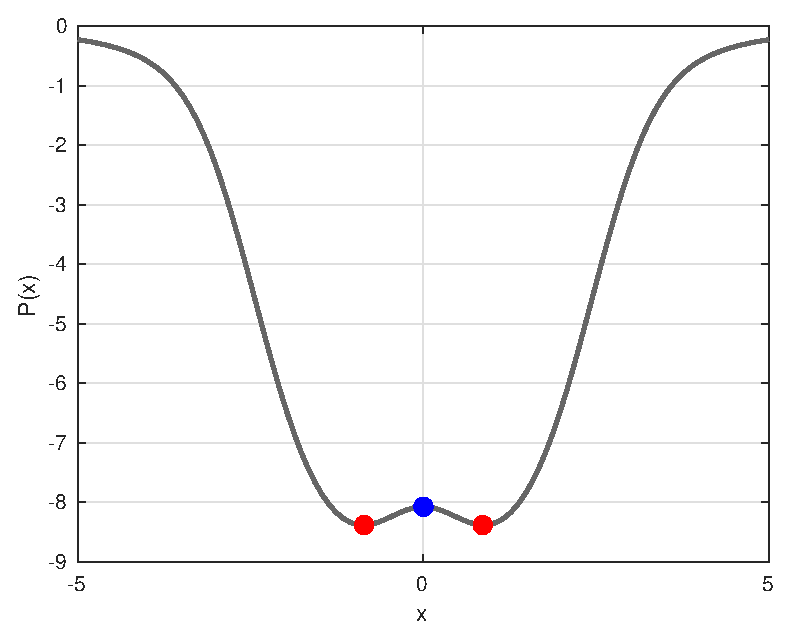
\includegraphics[scale=0.5]{img/Potential.eps} 
        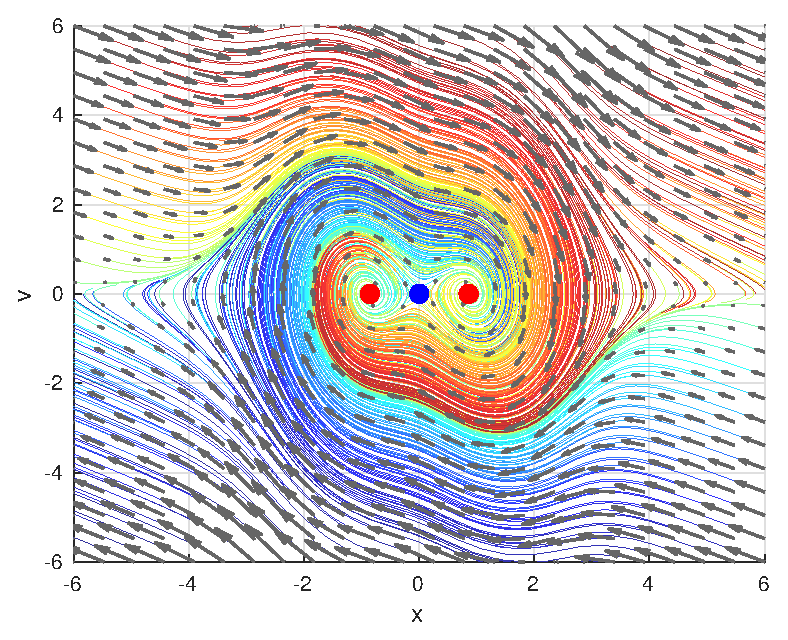
\includegraphics[scale=0.5]{img/pp_free.eps}
        \caption[Comportamiento de la partícula en un potencial]{
         A la izquierda se muestra el potencial en el que se mueve la partícula del ejemplo. Además a la derecha se muestra el comportamiento del espacio de fases del sistema. Alli estan dibujadas distintas trayectorias dentro del espacio de fases representadas con distintos colores. Podemos ver como todas las trayectorias acaban en los atractores representados por los puntos rojos, mientras que las trayectorias escapan del repulsor representado por el punto azul.}
        \label{fig:potencial}
    \end{figure}

    \begin{figure} 
        \centering
        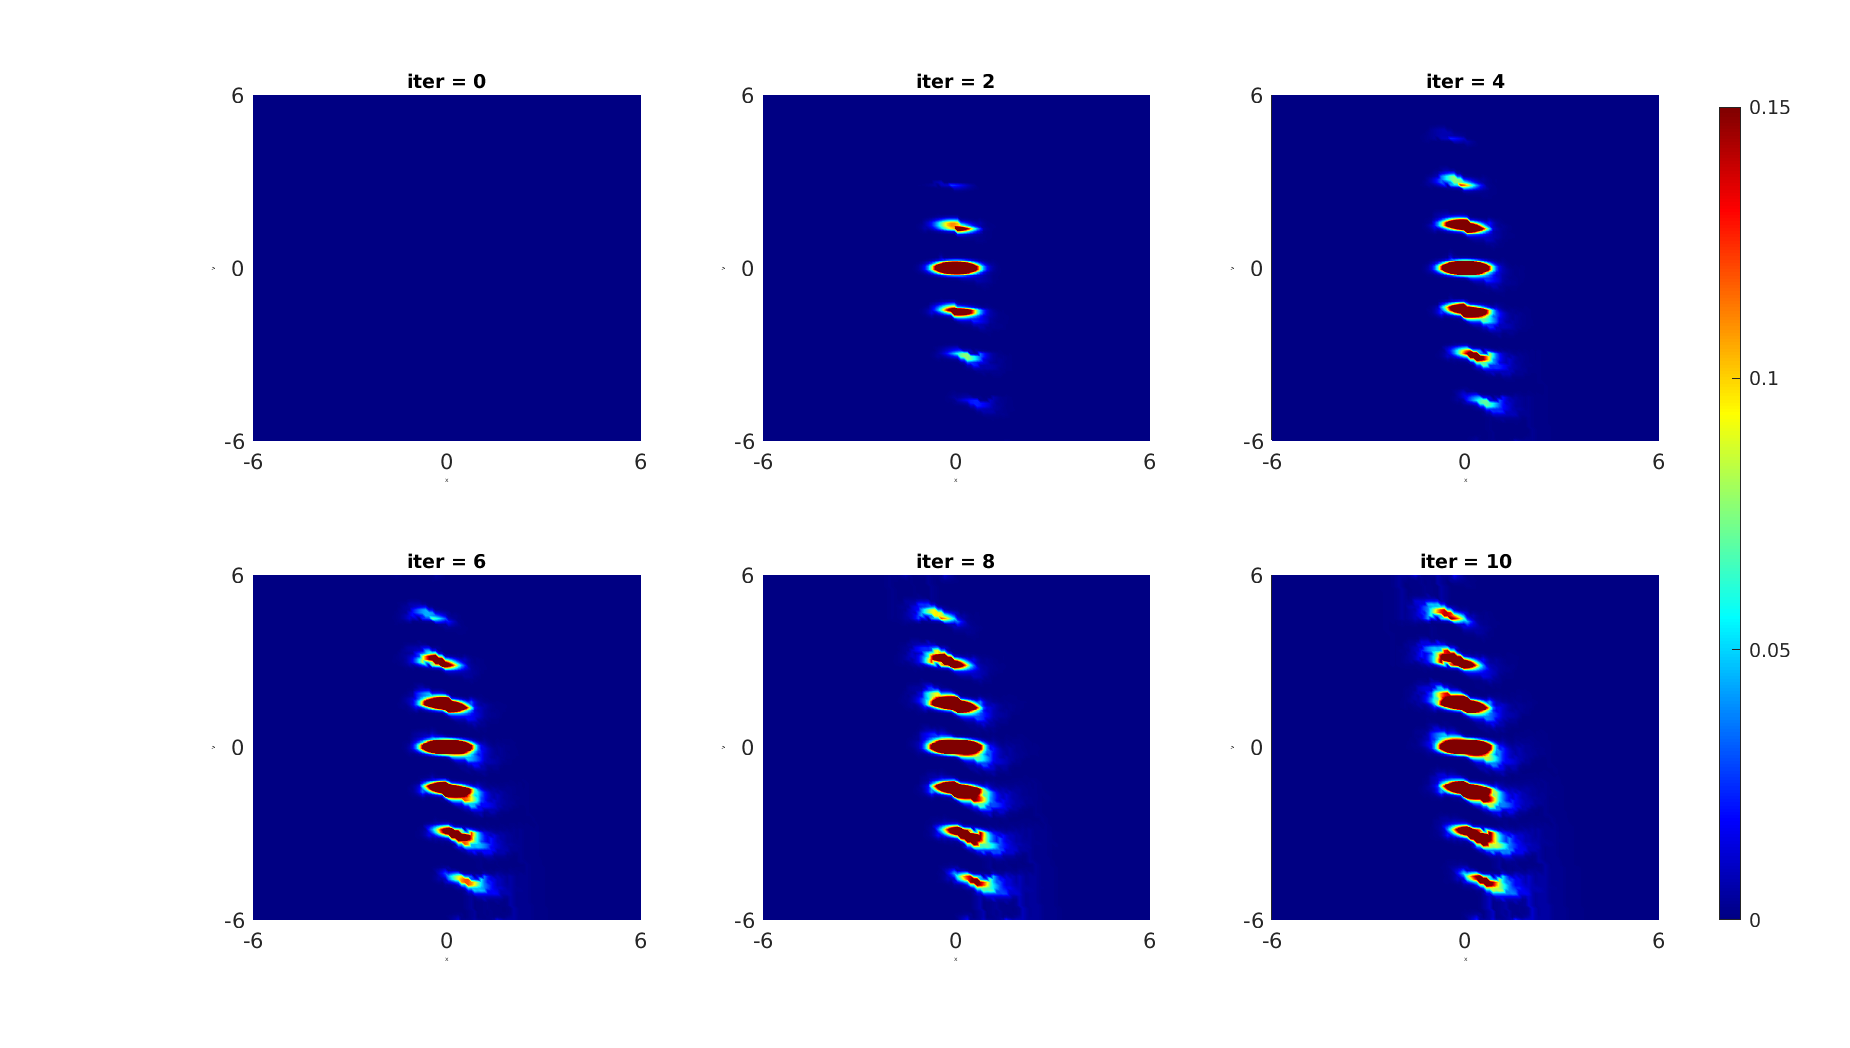
\includegraphics[scale=0.45]{img/valueiteration.eps}
        \caption[Evolución de la función vlaor por \emph{Value Iteration}]{Evolución de la función valor $\mathcal{V}_k(x,v)$ en distintas iteraciones del algoritmo  \emph{Q Iteration}. Podemos ver la convergencia de función valor de estado.}
        \label{fig:valueiteration}
    \end{figure} 

    \begin{figure} 
        \centering
        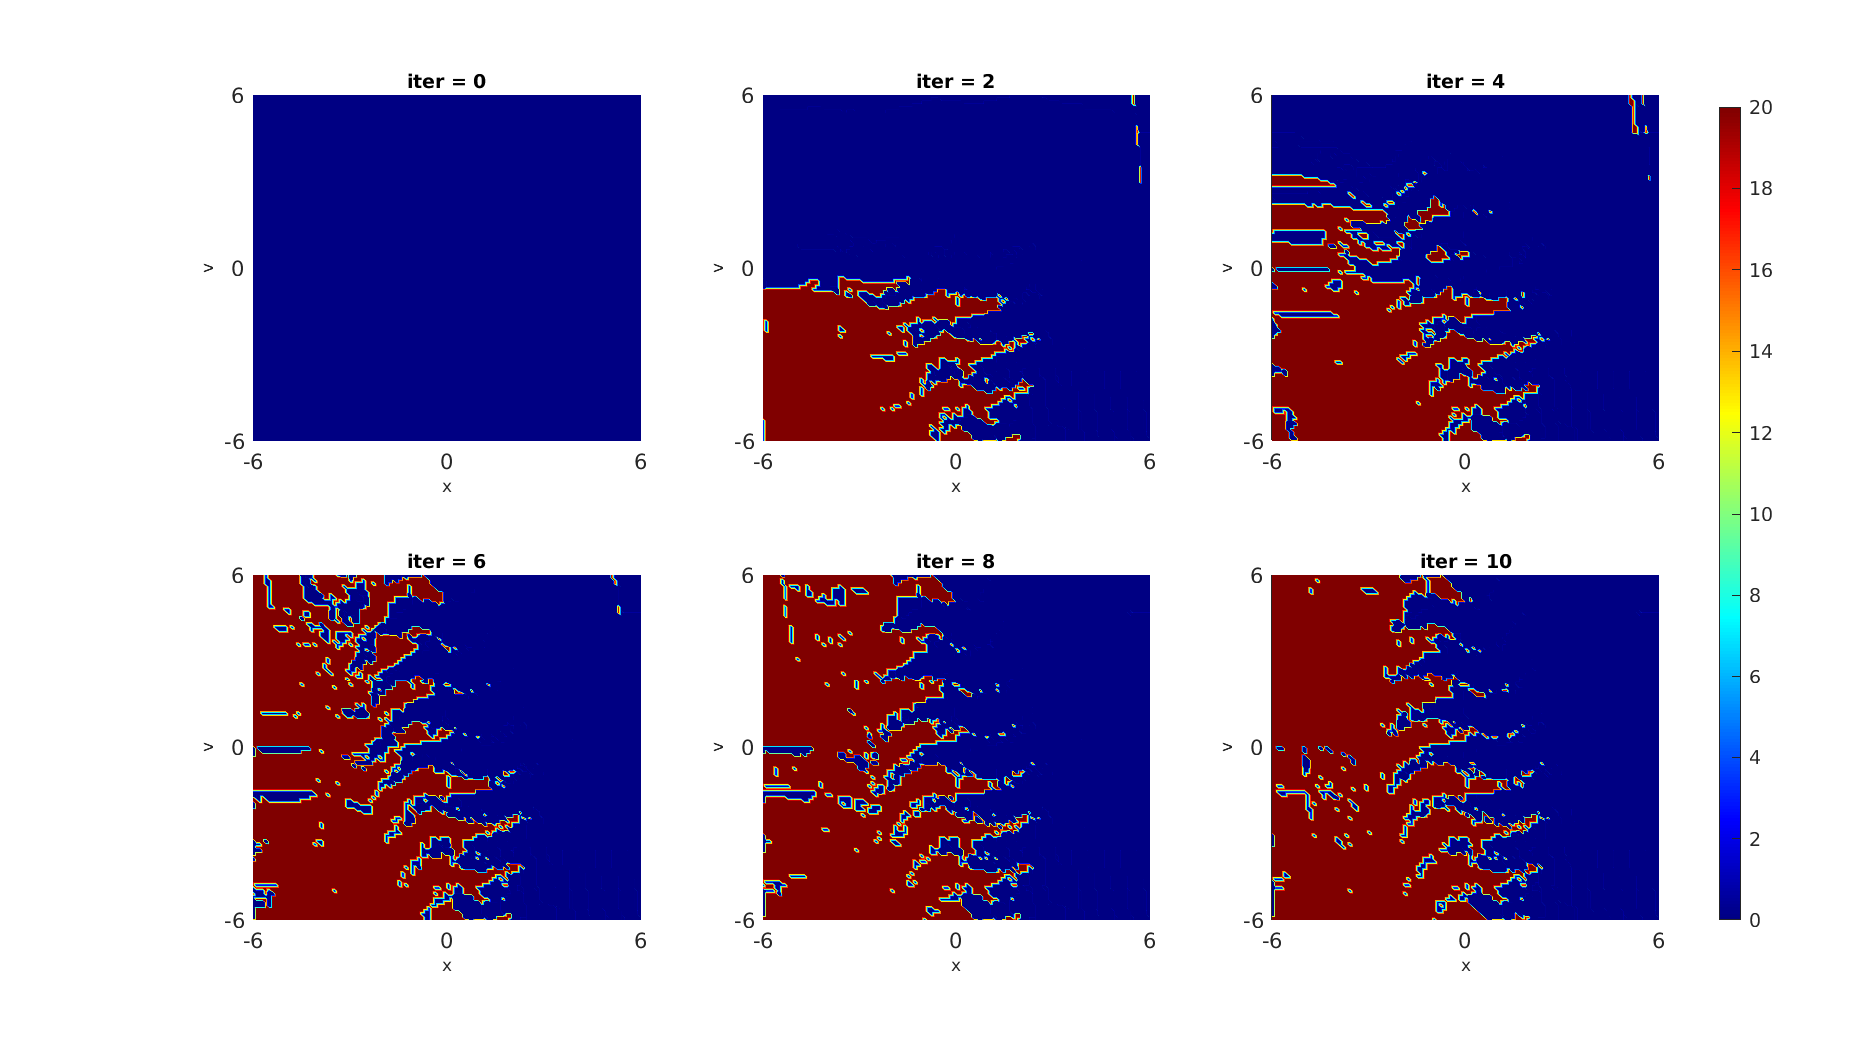
\includegraphics[scale=0.5]{img/valueiterationpi.eps}
        \caption[Evolución de la política por \emph{Value Iteration}]{
         Evolución de la política valor $\pi^*(x,v)$ en distintas iteraciones. Dado un punto del espacio de fases $(x,v)$ podemos obtener el valor de la acción. }
        \label{fig:piiteration}
    \end{figure} 

    \begin{figure}
        \centering
        \begin{subfigure}[b]{0.4\textwidth}
            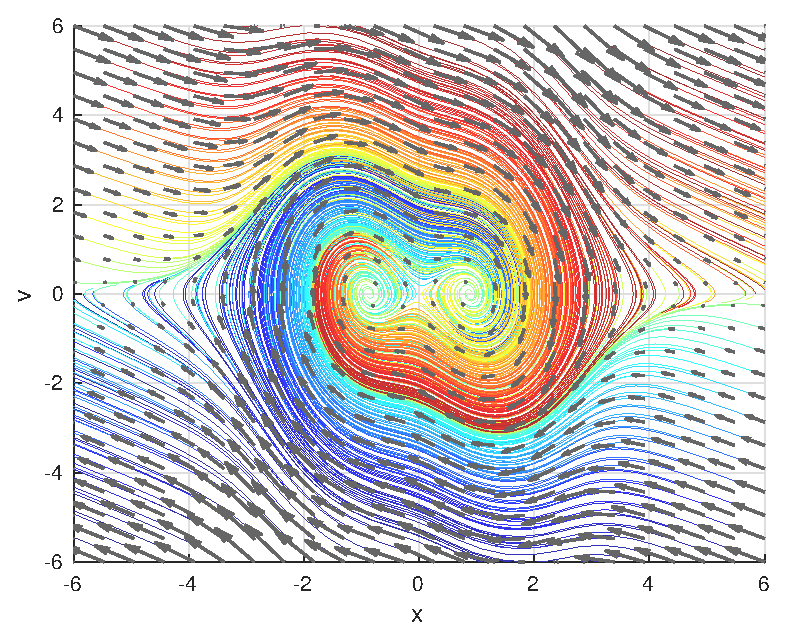
\includegraphics[width=\textwidth]{img/freepot.eps}
            \caption{Espacio de fases sin control}
            \label{afree}
        \end{subfigure}
        \begin{subfigure}[b]{0.4\textwidth}
            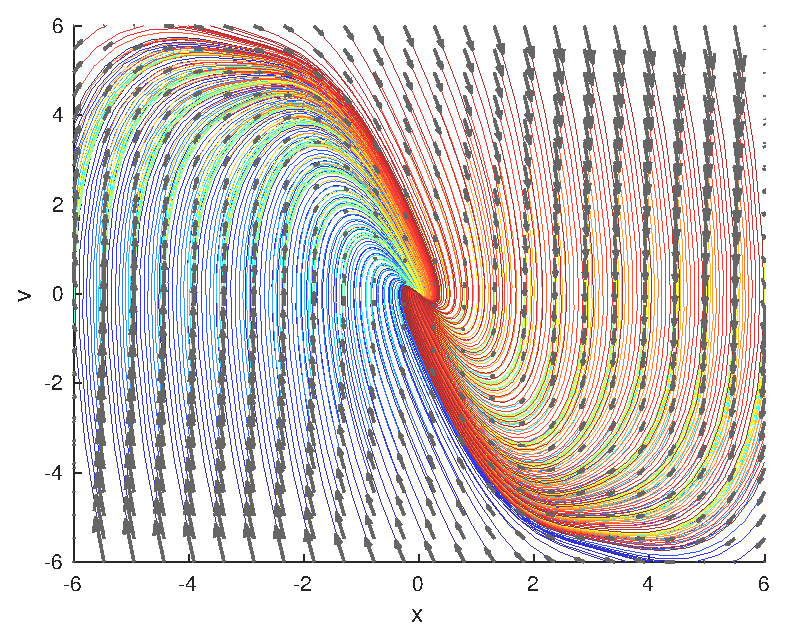
\includegraphics[width=\textwidth]{img/lqrpot.eps}
            \caption{Espacio de fases con LQR}
            \label{bLQR}
        \end{subfigure}
        \begin{subfigure}[b]{0.4\textwidth}
            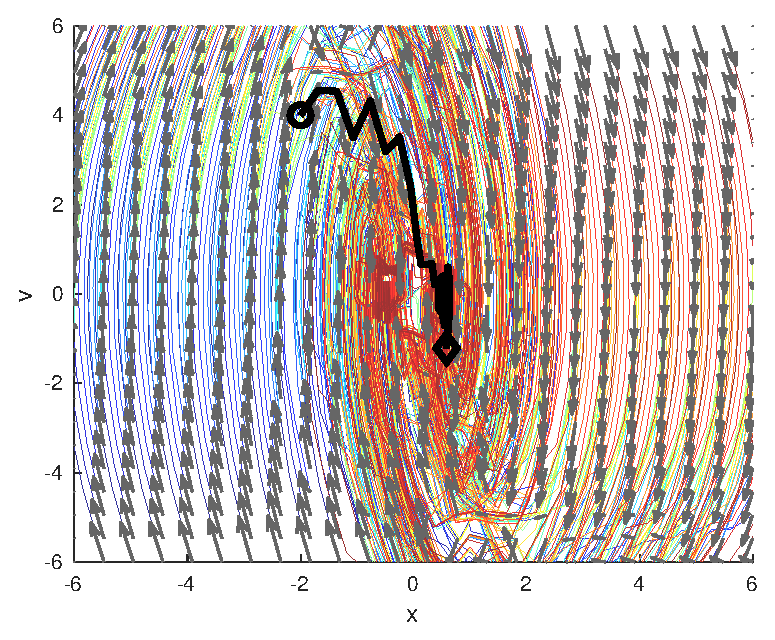
\includegraphics[width=\textwidth]{img/solpot.eps}
            \caption{Espacio de fases con \emph{Value Iteration}}
            \label{cQI}
        \end{subfigure}
        \begin{subfigure}[b]{0.4\textwidth}
            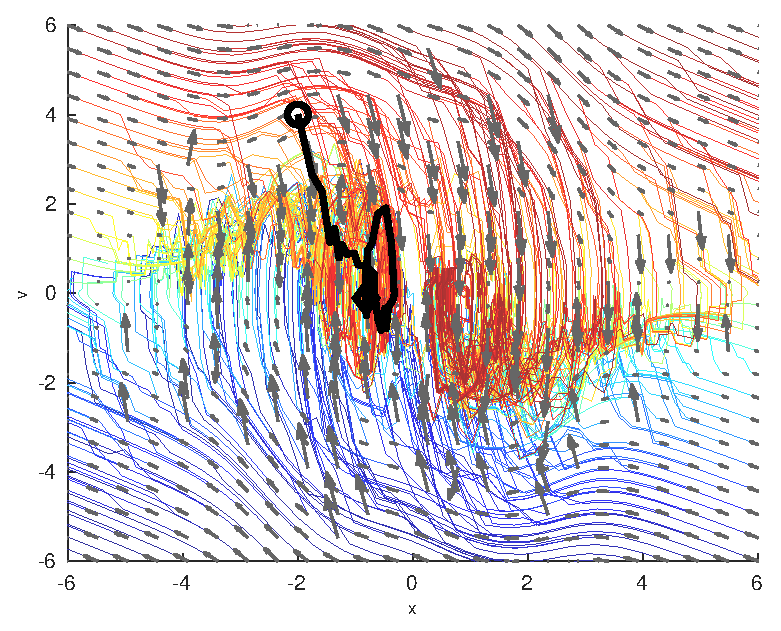
\includegraphics[width=\textwidth]{img/phase_Qlearning.eps}
            \caption{Espacio de fases con \emph{Q learning}}
            \label{cQI}
        \end{subfigure}
        
        \caption[Espacio de fases modificado]{
        Comparamos el espacio de fase del sistemas con la política obtenida mediante LQR (figura \ref{bLQR}), la política obtenida mediante el algoritmo \emph{Q-Iteration}  (figura \ref{cQI})y la dinámica libre (figura \ref{afree}).  }
        \label{fig:potencial}
    \end{figure}

\end{example}

%%%%%%%%%%%%%%%%%%%%%%%%%%%%%%%%%%%%%%%%%%%%%%%%%%%%%%%%%%%%%%%%%%%%%%%%%%%%%%%%%%%%%%%%%%%%%%%%%%%%%%%%%%%%%%%%%%%%%%%
%%%%%%%%%%%%%%%%%%%%%%%%%%%%%%%%%%%%%%%%%%%%%%%%%%%%%%%%%%%%%%%%%%%%%%%%%%%%%%%%%%%%%%%%%%%%%%%%%%%%%%%%%%%%%%%%%%%%%%%
%%%%%%%%%%%%%%%%%%%%%%%%%%%%%%%%%%%%%%%%%%%%%%%%%%%%%%%%%%%%%%%%%%%%%%%%%%%%%%%%%%%%%%%%%%%%%%%%%%%%%%%%%%%%%%%%%%%%%%%


\chapter{Introdución a Sistemas de recomendación}

% 
Un sistema de recomendación es un sistema de filtrado, capaz de predecir puntación que este da a un conjunto de elementos. El objetivo de estos sistemas es el proporcionar elementos con la mayor relevancia. 

En este capítulo introduciremos algunos sistemas de recomendación mencionando sus ventajas y desventajas, además de motivar el uso de la modelización de un sistema de recomendación como un proceso oculto de Markov. Luego formulalemos matemáticamente el sistema de recomendación, para además de resolverlo y realizar pruebas experimentales.


Existen varios tipos de sistemas de recomendación, a continuación mencionamos un clasificación representativo de estos.

\section{Filtrado colaborativo} 

En los sistemas de filtrado colaborativo \cite{schafer2007collaborative}, las puntaciones predichas de los elementos se calculan mediante la valoración de otros usuarios.  Suponiendo que tenemos una base de datos de $n$ usuarios y $m$ elementos a recomendar, los sistemas de recomendación colaborativo almacenan las puntaciones en una matriz $P \in \mathcal{M}_{n\times m}$. De esta forma, un elemento de la matriz $P{ij}$, corresponde a la puntación que el usuario $i$ da al elemento $j$. Deberemos notar que esta matrix $P$ no es completamente conocida sino que tiene muchos elementos desconocidos.  De esta manera, el problema de recomendación se traduce a descubrir la totalidad esta matriz $P$.
 
    \begin{itemize}
        \item \textbf{Ventajas}
        \begin{itemize}
            \item Interpretación de los resultados.
            \item Fácil implementación.
        \end{itemize} 

         \item \textbf{Desventajas} 
         \begin{itemize}
             \item Depende de las puntuaciones subjetiva de las personas.
             \item Su rendimiento disminuye cuando los datos son dispersos.
         \end{itemize}
    \end{itemize}

\section{Filtrado basado en contenido} 
    
    Los sistemas de recomendación basado en contenido \cite{lops2011content} se utilizan el historial del usuario como base del proceso. Los elementos del conjunto de recomendación tienen asociado un vector de carácteristicas. Por ejemplo, en el contexto de un sistema de recomendación de películas, un elemento puede ser de distinto género o duración, estas características son codificadas en un vector de $\mathbb{R}^d$, donde $d$ es el número de características consideradas. El usuario en estos sistemas elige las peĺiculas según sus gustos por lo que va escogiendo un conjunto de vectores que definen un subespacio vectorial. Entonces se considera una buena recomendación al elemento que más cerca este en el subespacio definido por el historial del usuario. 

    \begin{itemize}
        \item \textbf{Ventajas} 
        \begin{itemize}
            \item Independencia de Usuarios. Las recomendaciones solo dependen del perfil de usuario, por lo que se considera un solución personalizada.
            \item No es necesario que ningún usuario haya evaluado un elemento nuevo.
        \end{itemize}
        \item \textbf{Desventajas}
        \begin{itemize}
            \item Sobreespecialización. Cuando el historial del usuario es muy grande la solución de este sistema puede llegar a una configuración estacionaria, por lo que podemos llegar a recomendaciones siempre iguales
            \item Nuevo usuario. Es necesario que el historial del usuario sea suficientemente representativo para poder realizar recomendaciones fiables.
        \end{itemize}
    \end{itemize}

\section{Sistema de basado en un proceso de decición de Markov}
    En \cite{shani2005mdp} se describe el procesos de recomendación como un proceso de descisión de Markov. El usuario se considera un sistema dinámico, en donde el estado viene representado por una secuencia de elementos que ha seleccionado. Además las acciones a tomar viene represetnado por la siguiente recomendación. Es decir, se considera que la siguiente recomendación depende de el historial reciente del usuario. 
    
\begin{itemize}
    \item \textbf{Ventajas} 
    \begin{itemize}
        \item Solución dinámica. Un sistema de decomendación basado en un proceso de Markov puede a una solución que depende del estado actual del usuario, dado que este \emph{estado} puede variar en el tiempo la recomendación es dinámico.
    \end{itemize}
    \item \textbf{Desventajas}
    \begin{itemize}
        \item Gran necesidad de datos. Dado que la estimación se realiza mediante la máxima verosimilitud, esta necesita una gran cantidad de datos-
    \end{itemize}
\end{itemize}


En \cite{shani2005mdp} su validación se realiza a tiempo real mediante la interacción con usuarios reales por lo que no es necesario la simulación del usuario. En este trabajo proponemos una manera de utilizar el historial del usuario para la simulaciíon y además para dar una mejor inicialización al algoritmo de \emph{Q-learning}.
\chapter{Preprocesado del historial de películas}

Tomaremos como ejemplo la base de datos \emph{movieslens}\footnote{\url{<http://grouplens.org/datasets/>}}, publicada en \cite{MovieLens}. Esta base de datos describe la calificación de 5 estrellas un servicio de recomendación de películas. Contiene 100836 clasificaciones en 9742 películas. Estos datos fueron creados por 610 usuarios entre el 29 de marzo de 1996 y el 24 de septiembre de 2018. Este conjunto de datos se generó el 26 de septiembre de 2018. Todos los usuarios seleccionados habían calificado al menos 20 películas. 

A continuación explicaremos los pasos realizados para la obtención del historial de usuario, y luego explicaremos como agregaremos información para que sea posible el analisis de un sistema de recomendación


\section{Descripción de la base de datos iniciales}


Los datos están contenidos en las bases de datos: 
\begin{db}[movies.csv]\label{movies}
    Esta es una base de datos donde se describe enlaza el identificador numérico de la película con el nombre y los generos a los que pertenece. A continuación se describe las variables de esta base de datos:
    
    \begin{center}
        \begin{tabular}{|c|c|c|c|c|}
        \hline
        \textbf{Variable} & \textbf{Descripción} & \textbf{Tipo} & \textbf{Ejemplo 1} & \textbf{Ejemplo 2} \\ 
        \hline
         movieId & identificador & numérico & 1 & 3431 \\  
         title & nombre  & string & 
                Toy Story (1995)  & 
                Braveheart (1995)    \\
         genres & generos  & string & Comedy|Horror & Comedy|Drama|Romance \\
         \hline
        \end{tabular}
    \end{center} 
    \hfill$\square$
\end{db}

\begin{db}[ratings.csv]\label{ratings}
    Esta es una base de datos donde se registra para cada usuario y cada película que ha visto, la puntación que ha dado. A continuación se describe las variables de esta base de datos:
    \begin{center}
        \begin{tabular}{|c|c|c|c|c|}
        \hline
        \textbf{Variable} & \textbf{Descripción} & \textbf{Tipo} & \textbf{Ejemplo 1} & \textbf{Ejemplo 2} \\ 
        \hline
         userId & identificador de usuario   & numérico & 311 & 3431 \\  
        \hline
         movieId & identificador de película & numérico & 54 & 23 \\
        \hline
         rating & puntación  & numérico & 3 & 5 \\
        \hline
        timestamp & instante de tiempo  & numérico & 964983815 & 864913515 \\        
         \hline
        \end{tabular}
    \end{center} 
    \hfill$\square$
\end{db}

\section{Union de base de datos de generos y puntaciones}
Dado que queremos ver una recuerencia en el comportamiento de los usuario es muy dificil predecir las películas de manera indivudual. Podemos preguntarnos cuantas veces el usuario va a volver a mirar la misma película. Dado que la respuesta es muy pocas, los datos de entrenamiento para la predicción de la pélicula serán muy pequeñas. Si pensamos en una película como un elemento perteneciente a un espacio vectorial de caráterísticas podemos tener más datos de entrenamiento. Por esta razón, utilizando las bases de datos (\ref{movies}) y(\ref{ratings}) creamos la base de datos (\ref{moviesref})

\begin{db}[movies\_features.csv]\label{moviesref}
Esta base de datos contiene las películas disponibles para recomendar. Cada registro de la base de datos contiene el identificador y los generos que a los que puede pertener las películas

\begin{center}
    \begin{tabular}{|c|c|c|c|c|c|c|}
    \hline
    \textbf{Variable} & \textbf{Descripción} & \textbf{Tipo} & \textbf{Ejemplo 1} & \textbf{Ejemplo 2} \\ 
    \hline
    movieId & numérico   & Identificador &    12 &  143     \\
    \hline
    title   & string     & Nombre &    "Toy Story (1995)" &  "Jumanji (1995)"     \\
    \hline
    (no genres listed)  & ¿pertenece? & boleano &  1 &  0      \\
    Action              & ¿pertenece? & boleano &  1 &  0     \\
    Adventure           & ¿pertenece? & boleano &  1 &  0      \\
    Animation           & ¿pertenece? & boleano &  1 &  0      \\
    \dots & \dots                     &  \dots &  \dots &  \dots    \\
   \hline
    \end{tabular}
\end{center}
   \hfill$\square$
\end{db}

\section{Normalización de puntación de las película}

Dado que la puntación de las películas es subjetiva, normalizaremos las puntaciones de cada usuario de manera que la peor película valorada dentro de la base de datos para cada usuario tendrá la puntación $-1$, mientras que la mejor valorada tendrá el valor de $+1$. De esta forma, evitamos la sobrevaloración o subvaloración de las películas dependiendo del usuario


\begin{db}[ratings\_norm.csv]\label{ratingsnorm}
    Esta es una base de datos (\ref{ratings}) pero donde la puntación para cada usuario esta normalizada.
    \begin{center}
        \begin{tabular}{|c|c|c|c|c|}
        \hline
        \textbf{Variable} & \textbf{Descripción} & \textbf{Tipo} & \textbf{Ejemplo 1} & \textbf{Ejemplo 2} \\ 
        \hline
         userId & identificador de usuario   & numérico & 311 & 3431 \\  
        \hline
         movieId & identificador de película & numérico & 54 & 23 \\
        \hline
         rating & puntación  & numérico & -1 & 1 \\
        \hline
        timestamp & instante de tiempo  & numérico & 964983815 & 864913515 \\        
         \hline
        \end{tabular}
    \end{center} 
    \hfill$\square$
\end{db}


\begin{obs}
    En un entorno real esta normalización no es posible debido a que no podemos saber \emph{a priori} cual será la mayor puntación que dará un usuario. En un momento dado tendremos una puntación maximan y otra minima pudiendo escalar las puntaciones. Sin embargo si en alguna iteración este máximo o minimo cambia cambiarán todas las puntaciones relativas, complicando el problema. Aunque en esta tesis no consideramos este paso, deberemos notar que en un entrono real este problema será importante.
\end{obs}


\section{Componentes principales para generos de películas}

En esta base de datos (\ref{moviesref}) tenemos 24 generos de películas. Esta forma de clasificar las películas no tiene por que se la óptima a la hora de carácterizar cada película. Con el fin de reducir la dimensionalidad de la representación de cada película, procederemos al analisis de componentes principales. Esto lo realizaremos con ayuda de la función \verb|pca()| perteneciente a la biblioteca (\cite{MATPCA}).

Nos quedaremos con las primeras componentes principales que nos den una variabilidad explicada del 90\%. En este caso en la figura (\ref{VarExp}), se puede ver que el número de componentes principales para que esta condición se cumpla es $11$.De esta manera podemos tranformar la base de datos (\ref{moviesref}) a la base de datos (\ref{movierefPCA}).

\begin{figure}[ht!]
    \centering
    \begin{subfigure}[b]{0.4\textwidth}
        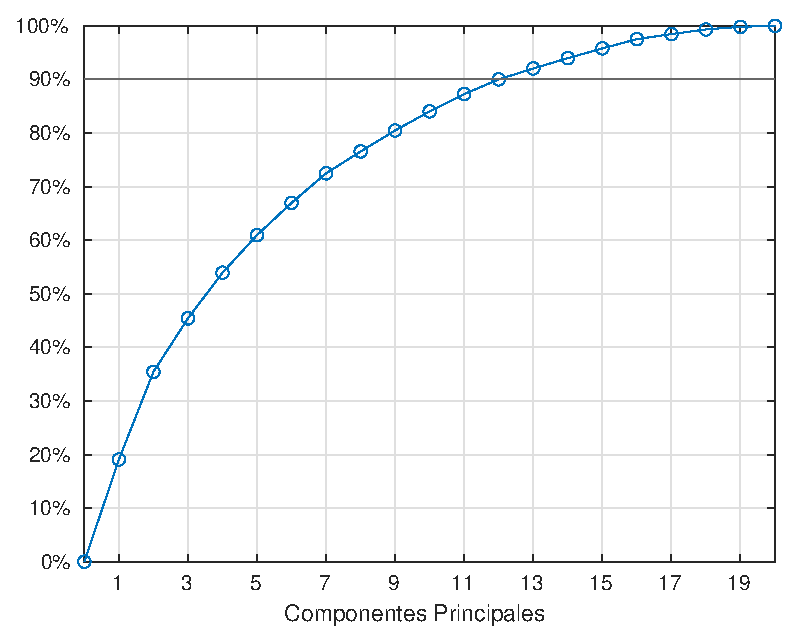
\includegraphics[scale=0.6]{img/varexp.eps}
        \caption{Variabilidad Explicada}\label{VarExp}
    \end{subfigure}
    \hspace{2cm}
    \begin{subfigure}[b]{0.4\textwidth}
        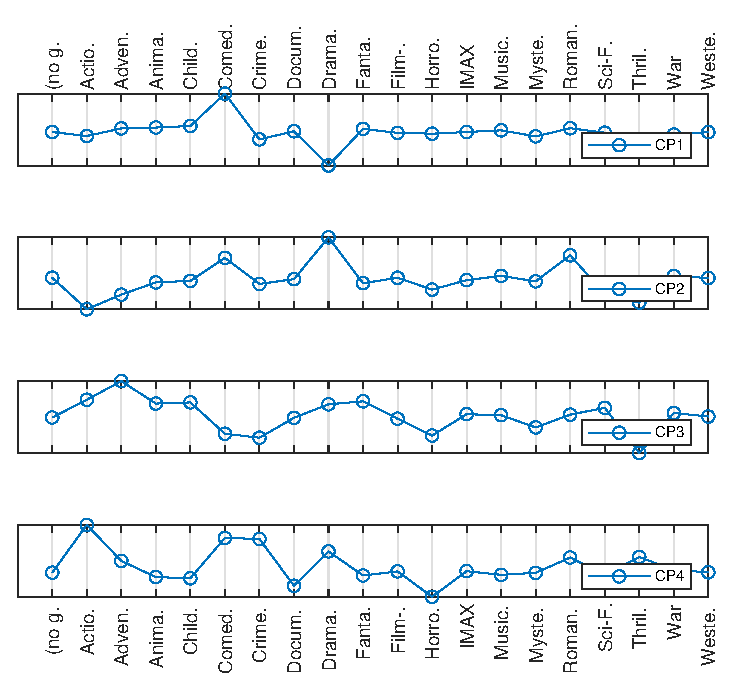
\includegraphics[scale=0.625]{img/firstPCA.eps}
        \caption{Primeras componentes}
    \end{subfigure}
    \caption{Analisis PCA en los generos de películas}
    \label{}
\end{figure}

\begin{db}[movies\_pca.csv]\label{movierefPCA}
    Esta base de datos con las componentes principales
    \begin{center}
        \begin{tabular}{|c|c|c|c|c|c|c|}
        \hline
        \textbf{Variable} & \textbf{Descripción} & \textbf{Tipo} & \textbf{Ejemplo 1} & \textbf{Ejemplo 2} \\ 
        \hline
        movieId & numérico   & Identificador &    12 &  143     \\
        \hline
        title   & string     & Nombre &    "Toy Story (1995)" &  "Jumanji (1995)"     \\
        \hline
        PC01  & Coordenada & numérico &  0.1 &  -0.3      \\
        PC02  & Coordenada & numérico &  0.5 &  0.1     \\
        PC03  & Coordenada & numérico &  1.0 &  1.0      \\
        \dots & \dots                     &  \dots &  \dots &  \dots    \\        PC11  & Coordenada & numérico &  4.0 &  -3.1      \\
       \hline
        \end{tabular}
    \end{center}
    \hfill $\square$
\end{db}


\section{Historial de aceptación para cada usuario}


Para ello, cruzaremos la base de datos \emph{movies.csv} y \emph{rating.csv}, para crear una nueva base de datos que en sus variables contenga cada uno de los generos disponibles en la totalidad de los datos. 

\begin{db}[user\_movies\_accept.csv]\label{user_movies_features}
    Esta es una base de datos que registra las interacciones de distintos usuarios con las distintas películas, además de informar del vector de caráterísticas de cada película vista.
    \begin{center}
        \begin{tabular}{|c|c|c|c|c|}
        \hline
        \textbf{Variable} & \textbf{Descripción} & \textbf{Tipo} & \textbf{Ejemplo 1} & \textbf{Ejemplo 2} \\ 
        \hline
            userId & identificador de usuario   & numérico & 311 & 3431 \\  
        \hline
            rating & puntación  & numérico & 3 & 5 \\
        \hline
        timestamp & instante de tiempo  & numérico & 964983815 & 864913515 \\        
        \hline
        PC01  & Coordenada & numérico &  0.1 &  -0.3      \\
        PC02  & Coordenada & numérico &  0.5 &  0.1     \\
        PC03  & Coordenada & numérico &  1.0 &  1.0      \\
        \dots & \dots                     &  \dots &  \dots &  \dots    \\        PC11  & Coordenada & numérico &  4.0 &  -3.1      \\
            \hline
        \end{tabular}
    \end{center}
    \hfill$\square$         
\end{db}



Si consideramos que tenemos $d$ géneros, entonces para cada usuario tenemos una secuencia de vectores $\bm{x}_t \in [0,1]^d \ | \ \forall t \in \{ 1,\dots,T\}$. Por último, si una película pertenece a varios géneros a la vez, el módulo del vector asociado será más grande que una película con menos géneros asociados. Dado que el módulo de un vector puede afectar a los modelos de prodicción normalizaremos todos los vectores $\bm{x}_d$. 

Asi pues, el historial de un usuario se puede entender como la rotación de un vector $\bm{x}_t$:

\begin{gather}
    \{ \bm{x}_t  \}_{t \geq0} \in \mathbb{R}^d \ \ | \ ||\bm{x}_t|| = 1 \ \forall t \leq 0
\end{gather}



\section{Generación sintética del historial de rechazo}

El problema que tenemos en estos datos es que solo tenemos las películas que el usuario ha seleccionado en cada iteración, sin embago si consideramos el proceso de recomendación en cada iteración el usuario se le ha recomendado una serie de peliculas de las cuales solo tenemos constancia la película que ha seleccionado. Es por ello que consideraremos que en cada iteración el sistema de recomendación a ofrecido dos películas al usuario. Una de ella la ha aceptado y la otra la ha rechazado. Para crear el historial de películas rechazadas agregaremos de manera ficticia otra película que tengamos en el historial del usuario pero que tenga menor puntación que la película que ha selecionado en la realidad. 

\begin{db}[user\_movies\_reject.csv]\label{user_movies_features_reject}
    Base de datos con la misma estructura y la mismas instancias que la base de datos (\ref{user_movies_features}), pero esta contiene las películas que el usuario ha rechazado.
    \begin{center}
        \begin{tabular}{|c|c|c|c|c|}
        \hline
        \textbf{Variable} & \textbf{Descripción} & \textbf{Tipo} & \textbf{Ejemplo 1} & \textbf{Ejemplo 2} \\ 
        \hline
            userId & identificador de usuario   & numérico & 311 & 3431 \\  
        \hline
            \st{rating} & -  & - & - & - \\
        \hline
        timestamp & instante de tiempo  & numérico & 964983815 & 864913515 \\        
        \hline
        PC01  & Coordenada & numérico &  0.1 &  -0.3      \\
        PC02  & Coordenada & numérico &  0.5 &  0.1     \\
        PC03  & Coordenada & numérico &  1.0 &  1.0      \\
        \dots & \dots                     &  \dots &  \dots &  \dots    \\        PC11  & Coordenada & numérico &  4.0 &  -3.1      \\
            \hline
        \end{tabular}
    \end{center}
    \hfill $\square$
\end{db}
\begin{obs}
    Para el historial de aceptación tambien tenemos su correspondiente puntación, sin embargo para el historial de rechazos dado que el usuario no lo ha selecionado, en general no tenemos puntación asociada.
\end{obs}


    


\section{Bases de datos finales: Historiales de usuarios}\label{HObt}


En la figura (\ref{DFPrePro}) mostramos un diagrama de flujo de como hemos creado los historiales de usuario que finalmente se utilizarán para entrenar un proceso de deción de Markov. 

Finalmente para cada usuario tenemos: el historial de películas aceptadas y el historial de rechazadas.
\begin{itemize}
    \item Tenemos la acciones en cada iteración: 
    \begin{gather}
        \{\bm{a}_t\}_{t\geq 0} =\{ \bm{x}_t^a,\bm{x}_t^r\}_{t\geq 0}
    \end{gather}

    \item Tenemos el estado en cada iteración: 
    \begin{gather}
        \{\bm{s}_t\}_{t\geq 0} = \{ \bm{x}_t^a\}_{t \geq 0}
    \end{gather}

    
\end{itemize}

Denotaremos al historial de un usuario como 
\begin{gather}
    \mathcal{H} = \{ \bm{x}_t^r,\bm{x}_t^a\}_{t \geq 0}
\end{gather}
 
Mostramos como ejemplo la siguiente tabla como historial de aceptación (base de datos \ref{user_movies_features}):
\begin{center}
    \begin{tabular}{|c|c|c|c|c|c|c|}
\hline
\textbf{title}          &              \textbf{rating}  &  \textbf{timestamp}   &    \textbf{Action}   &  \textbf{Adventure} & \dots \\
\hline
"The Drop (2014)"                   &      2   &   1.4795e+09  &       0        & 0  & \dots \\  
"Django Unchained (2012)"           &    3.5   &   1.4795e+09  &       0.57735  & 0  & \dots \\ 
"Interstellar (2014)"               &      3   &   1.4795e+09  &       0        & 0  & \dots \\  
"The Drop (2014)"                   &      2   &   1.4795e+09  &       0        & 0  & \dots \\  
"The Drop (2014)"                   &      2   &   1.4795e+09  &       0        & 0  & \dots \\  
"Exit Through the Gift Shop (2010)" &      3   &   1.4795e+09  &       0        & 0  & \dots \\  
"Collateral (2004)"                 &    3.5   &   1.4795e+09  &       0.5      & 0  & \dots \\  
    \hline
    \end{tabular}
\end{center}

Además del historial de rechazo (base de datos \ref{user_movies_features_reject}):

\begin{center}
    \begin{tabular}{|c|c|c|c|c|c|c|}
\hline
\textbf{title}          &              \textbf{rating}  &  \textbf{timestamp}   &    \textbf{Action}   &  \textbf{Adventure} & \dots \\
\hline
"The Drop (2014)"                   &      2   &   1.4795e+09  &       0        & 0  & \dots \\  
"Django Unchained (2012)"           &    3.5   &   1.4795e+09  &       0.57735  & 0  & \dots \\ 
"Interstellar (2014)"               &      3   &   1.4795e+09  &       0        & 0  & \dots \\  
"The Drop (2014)"                   &      2   &   1.4795e+09  &       0        & 0  & \dots \\  
"The Drop (2014)"                   &      2   &   1.4795e+09  &       0        & 0  & \dots \\  
"Exit Through the Gift Shop (2010)" &      3   &   1.4795e+09  &       0        & 0  & \dots \\  
"Collateral (2004)"                 &    3.5   &   1.4795e+09  &       0.5      & 0  & \dots \\  
    \hline
    \end{tabular}
\end{center}



\tikzstyle{startstop} = [rectangle, rounded corners, minimum width=1.5cm, minimum height=1.cm,text centered, draw=black, fill=blue!30,line width=1.25pt]
%
\tikzstyle{cir} = [circle, rounded corners, minimum width=1.05cm, minimum height=0.5cm,text centered, draw=black, fill=green!30,line width=1.25pt]
%
\tikzstyle{cir_hd} = [circle, rounded corners, minimum width=0.5cm, minimum height=0.5cm,text centered, draw=black, fill=red!30,line width=1.25pt]
%%%%%%%%%%%%%%%%%%%%%%%%%%%%%%%%%%%%%%%%%%%%%%%
% for double arrows a la chef
% adapt line thickness and line width, if needed
\tikzstyle{vecArrow} = [thick, decoration={markings,mark=at position
   1 with {\arrow[semithick]{open triangle 60}}},
   double distance=1.4pt, shorten >= 5.5pt,
   preaction = {decorate},
   postaction = {draw,line width=2.4pt, white,shorten >= 4.5pt}]
\tikzstyle{innerWhite} = [semithick, white,line width=1.4pt, shorten >= 4.5pt]

\begin{figure}[]
    \centering
        
\begin{tikzpicture}[node distance=2.05cm] 
    \filldraw[color=red!60, fill=red!5, very thick](-1.7,1.4) rectangle (1.55,-2.7);
    \filldraw[color=blue!60, fill=blue!5, very thick](1.65,1.4) rectangle (8.2,-2.7);
    \filldraw[color=green!60, fill=green!5, very thick](8.30,1.4) rectangle (12.70,-2.7);

    \node[draw,fill=red!20] at   (-0.1,1.0) {\small \textbf{B.D. de Entrada}};
    \node[draw,fill=blue!20] at  (4.9   ,1.0) {\small \textbf{B.D. Intermedias}};
    \node[draw,fill=green!20] at (10.5   ,1.0) {\small \textbf{B.D de Salida}};



    \node (movies) [startstop] {\small movies.csv};
    \node (ratings) [startstop,below of=movies] {\small ratings.csv};

    \node (ratingsnorm) [startstop,right of=ratings,xshift=3cm] {\small ratings\_norm.csv};

    \node (moviesfeatures) [startstop, right of=movies,xshift=1.5cm] {\small movies\_features.csv};

    \node (moviespca) [startstop, right of=moviesfeatures,xshift=1cm] {\small movies\_pca.csv};

    \node (usermovies) [startstop,  right of=ratings,xshift=8.5cm] {\small user\_movies\_accept.csv};
    %
    \node (usermoviesreject) [startstop,above of=usermovies] {\small user\_movies\_reject.csv};
%%%%%
    \draw  [line width=1.25pt,bend left=0,<-] (moviesfeatures) edge (movies);
    \draw  [line width=1.25pt,bend left=0,<-] (moviespca) edge (moviesfeatures);
    \draw  [line width=1.25pt,bend left=10,<-] (usermovies) edge (moviespca);

    \draw  [line width=1.25pt,bend left=0,<-] (ratingsnorm) edge (ratings);
    \draw  [line width=1.25pt,bend left=0,<-] (usermovies) edge (ratingsnorm);

    \draw  [line width=1.25pt,bend left=0,<-] (usermoviesreject) edge (usermovies);

\end{tikzpicture}

    \caption{Diagrama de flujo para el preprocesado de los datos.}{En rojo las base de datos obtenidas de \cite{MovieLens}, en azul las bases de datos creadas como pasos Intermedias y finalmente en verde las bases de datos que se usarán en esta tesis.}
    \label{DFPrePro}


\end{figure}


\chapter{Sistema de recomendación como proceso de decisión de Markov }

En esta sección presentaremos un sistema de recomendación mediante una proceso de decisión de Markov y resolveremos el problema de recomendación mediante la metodología de aprendizaje por refuerzo.

\section{Proceso de  decisión de Markov}
Definimos una proceso de decisión de Markov inspirado en \cite{shani2005mdp}. Aunque distinto debido a caráteristicas de los datos disponibles.
\begin{itemize}
    \item \textbf{Estado}: Pelicula vista en el instante anterior. Es espacio donde vive este estado es: 
    \begin{gather}
        \Ss = \{ x \in \mathbb{R} \ \ | \ \  ||x|| = 1\}
    \end{gather}
    Donde $d$ es el número de generos considerados en la base de datos.
    \item \textbf{Acción}: Las dos películas que enseñamos al usuario. Entonces el espacio de acciones es 
    \begin{gather}
        \As = \{ \bm{a} \in \Ss \times \Ss \}
    \end{gather}
    \item \textbf{Recompenza}: Puntación que da a la película selecionada. Representado por $r_t \in [-1,1]$. Suponemos que este puede depender del estado $\bm{x}_t$ y de la acción $\bm{a}_t$, sin embargo no sabemos que forma funcional tiene.
    \item \textbf{Ecuación dinámica}: Tal como se ha creado la base de datos, sugiere que la dinámica del usuario puede escoger la película según la puntación asociada. Sin embargo, en el plantamiento el usuario hasta despues de ver la película no tiene una puntación asociada por lo que la puntación a \emph{priori} que tiene el usuario sobre dos películas es la que determina la eleción. Dado que en la metodología de aprendizaje por refuerzo no es necesario el conocimiento de la dinámica, no es necearia definirla.
\end{itemize}

Mostramos un esquema de la interación del usuario y el sistema de recomendación en la figura \ref{sqmrs}

\begin{obs}
    La acción en cada instante $t$ es un par de vectores $\bm{x}_1,\bm{x}_2 \in \mathbb{R}^d$, sin embargo en la realidad el sistema de recomendación deberá recomendar un título de película y no un vector de caráterísticas. Por esta razón, necesitamos una función que traduzca un vector de caráterísticas $\bm{x}$ en un titulo de la base de datos. Tomaremos como peliculas correspondiente a $\bm{x}$ la película más parecidad que tengamos en la base de datos y que no haya visto el usuario.
\end{obs}




\tikzstyle{startstop} = [rectangle, rounded corners, minimum width=1.5cm, minimum height=1.cm,text centered, draw=black, fill=blue!30,line width=1.25pt]
%
\tikzstyle{cir} = [circle, rounded corners, minimum width=1.05cm, minimum height=0.5cm,text centered, draw=black, fill=green!30,line width=1.25pt]
%
\tikzstyle{cir_hd} = [circle, rounded corners, minimum width=0.5cm, minimum height=0.5cm,text centered, draw=black, fill=red!30,line width=1.25pt]
%%%%%%%%%%%%%%%%%%%%%%%%%%%%%%%%%%%%%%%%%%%%%%%
% for double arrows a la chef
% adapt line thickness and line width, if needed
\tikzstyle{vecArrow} = [thick, decoration={markings,mark=at position
   1 with {\arrow[semithick]{open triangle 60}}},
   double distance=1.4pt, shorten >= 5.5pt,
   preaction = {decorate},
   postaction = {draw,line width=2.4pt, white,shorten >= 4.5pt}]
\tikzstyle{innerWhite} = [semithick, white,line width=1.4pt, shorten >= 4.5pt]

\begin{figure}[]
    \centering
    \hfill
    \begin{subfigure}[b]{0.4\textwidth}
        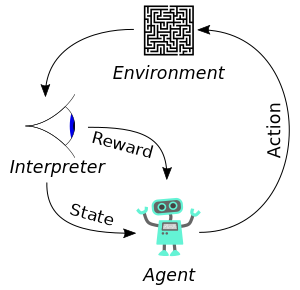
\includegraphics[scale=0.55]{img/Reinforcement_learning_diagram.png}
        \caption{Esquema estándar del aprendizaje por refuerzo \cite{WikiRF}}\label{fig:WikiRF}
        \label{afree}
    \end{subfigure}
    \hspace{0.4cm}
    \begin{subfigure}[b]{0.4\textwidth}
        \begin{tikzpicture}[node distance=2.05cm]
            \filldraw[color=red!60, fill=red!5, very thick](2.15,2.7) rectangle (6,-2.7);
            
            \node[draw,fill=red!20] at (2.9,2.35) {\footnotesize \textbf{Agente}};
    
            \filldraw[color=green!60, fill=green!5, very thick](-2.35,-2.7) rectangle (2.05,2.7);

            \node[draw,fill=green!20] at (-0.45,2.35) {\footnotesize \textbf{Ambiente e Intérprete}};

            \node (start) [startstop] {\footnotesize Usuario};
            \node (state) [cir,above of=start,yshift=-0.6cm] {$\bm{x}_{t-1}$};
            \node (action) [cir,right of=start,xshift=2.1cm,yshift=1.4cm] {$\bm{a}_{t}$};
            \node (reward) [cir,below right of=start] {$r_{t}$};
            \node (nextstate) [cir,below left of=start,] {$\bm{x}_{t}$};
    
            \node (RS) [startstop,below right of=reward,xshift=1.25cm,yshift=0.9cm] {$\text{\footnotesize S.  de  Recomendación}$}; 
    
            %
            \node (m2) [cir_hd,above of=RS,xshift=+1.0cm,yshift=-0.3cm] {$\text{\footnotesize pelíc.}_{2}$};
            \node (m1) [cir_hd,above of=RS,xshift=-1.0cm,yshift=-0.3cm] {$\text{\footnotesize pelíc.}_{1}$};
            %
            \draw  [line width=1.25pt,bend left=-70,<-] (state) edge (nextstate);
            \draw  [line width=1.25pt,bend left=0,<-] (start) edge (state);
            \draw  [line width=1.25pt,bend left=-35,<-] (nextstate) edge (start);
            \draw  [line width=1.25pt,bend left=+15,<-] (start) edge (action);
            \draw  [line width=1.25pt,bend left=35,<-] (reward) edge (start);
            %
            \draw  [line width=1.25pt,<-,bend left=-20] (action) edge (m1);
            \draw  [line width=1.25pt,<-,bend left=20] (action) edge (m2);
            %
            \draw  [line width=1.25pt,bend left=-25,<-] (m1) edge (RS);
            \draw  [line width=1.25pt,bend left=+25,<-] (m2) edge (RS);
            %
            %
            \draw  [line width=1.25pt,bend left=20,<-] (RS) edge (nextstate);
            \draw  [line width=1.25pt,<-,bend left=+5] (RS) edge (reward);
        \end{tikzpicture}
        \caption{Esquema específico de aprendizaje por refuerzo en el sistema de recomendación.}
        \label{sqmrs}
    \end{subfigure}
    \hspace{\fill}

    \caption{ Aprendizaje por refuerzo en el sistema de recomendación}
\end{figure}



\section{Plantamiento de los problemas}

En esta tesis buscarémos políticas para realizar buenas recomendaciones de manreda que la puntación acumuladad del usuario sea máxima. Este problema puede ser planteado desde el momento en el que el usuario empieza a usar el sistema de recomendación o cuando tenemos ya historial suficiente del usuario para poder inferir una manera de actuar. En el primero de ellos, dado que no tenemos ninguna información del usuario deberemos utilizar los datos de los usuarios anteriores. Acontinuación plantemos los dos problemas.


\begin{problem}[Sin historial]\label{prob1}
    Suponiendo que tenemos un historial de aceptación $\{ \bm{x}_t^a\}_{t\geq 0}$ y de rechazo $\{ \bm{x}_t^r\}_{t\geq 0}$ del usuario. ¿Cómo podemos obtener una política $\pi: \Ss \rightarrow \As $ que nos maximize la recompensa acumulada?
\end{problem}


\begin{problem}[Con historial]\label{prob2}
    Suponiendo que tenemos un base de datos de historial de aceptación $\{ \bm{x}_t^a\}_{t\geq 0}$ y rechazo de varios usuarios $\{ \bm{x}_t^r\}_{t\geq 0}$, pero no tenemos historial del usuario al que se le va a recomendar. ¿Cómo podemos obtener una política $\pi: \Ss \rightarrow \As $, que nos maximize la recompensa acumulada?
\end{problem}







\section{Metodología}

En esta sección describiremos los pasos que se ha seguido para abordar los problema planteados en la sección anterior.

\subsection{Selección de estado inicial}

Dado que la condición incial se determina por una primera recomendación que no nos es posible determinar lo tomaremos como aleatorio. Luego buscaremos la política óptima que nos permita encontrar los datos de entrenamiento. 

\subsection{Inicialización de la función valor estado-acción}\label{InitQ}

En cierto momento tenemos un historial de usuario, hacemos \emph{Q-learning} mediante las acciones que tenemos disponibles. En \cite{fujimoto2019off}, se estudia el problema de aprendizaje por refuerzo cuando tenenemos los datos ya dados. Alli se ve que la convergencia del algoritmo \emph{Q-learning} dentro de un conjunto de datos ya dados tambien converge a la política óptima.

\begin{thm}
    \cite{fujimoto2019off}. \textit{La realización de Q-learning mediante el muestreo de un conjunto de datos $B$ converge a la función valor óptimo.}
\end{thm}

Entonces 
\begin{gather}
    Q(s,a) \leftarrow (1-\alpha)Q(s,a) + \alpha \bigg( r +\gamma \max_{a' s.t (s',a') \in \mathcal{B}} Q(s',a') \bigg)
\end{gather}

\begin{algorithm}[!ht]
    \caption{\emph{Batch Q-learning }}\label{Qlearning}
    \begin{algorithmic}[1]
        \Procedure{Bacth Q-learning}{$\mathcal{Q}^{*},s_0,tol,\alpha,\epsilon$}
        \State $k \gets 0$
        \State $\mathcal{Q}_1 \gets \mathcal{Q}^{*}$
        \While{$ error \leq tol$}
            \State $k \leftarrow k + 1$
            \State Sample $(s_t,a_t,s_{t+1},r_t)$
            \State $\displaystyle \mathcal{Q}_k(s_t,a_t) \gets (1-\alpha)\mathcal{Q}_{k-1}(s_t,a_t) +  
            \big[ r_t + \gamma \max_{a'\in \As \ s.t.(s_{t+1},a')  \in \mathcal{B} \ }\mathcal{Q}_{k-1}(s_{t+1},a') \big]$
            \State $error=|| Q_k - Q_{k+1}||^2$

        \EndWhile
        \State \textbf{return} $\{a_t\}_{t>0}$
        \EndProcedure
    \end{algorithmic}
\end{algorithm}


La evaluación de la política se realizará mediante el uso de los datos restantes. Para ello se selecionará la acción óptima como la acción que nos mande la política encontrada, proyectado a los datos que tengamos en los datos restantes.

\begin{enumerate}
    \item \textbf{Con historial(Problema \ref{prob1})}. Tomaremos como datos de entrenamiento el historial del propio usuario.
    \item \textbf{Sin historial(Problema \ref{prob2})}. Tomaremos como datos de entrenamiento todo el conjunto de usuario suponiendo que todas las interacciones de la base de datos provienen 
\end{enumerate}

\subsection{Política utilizada}

Utilizaremos la metodología de \emph{Q-learning} inicializando la función valor estado-acción como se ha mencionado en la sección (\ref{InitQ})


\subsection{Selección de peliculas  desde un política dada}

Dividiremos la base de datos generada en la sección (\ref{HObt}). Teniendo en cuenta todos los usuarios ordenaremos temporalmente los datos $\{\bm{x}_t^r,\bm{x}_t^a\}$  para todos los usuarios y lo dividiremos por la mitad. De esta forma, existirán algunos usuarios que no hayan interacionado con el sistema de recomendación en toda la base de datos de entrenamiento y otros de los cuales si se tenga historial. De esta manera, podemos probar los problemas (\ref{prob1}) y (\ref{prob2}).

Entonces para un usuario tenemos 
\begin{enumerate}
    \item \textbf{Una historial de entrenamiento}: Para cada usuario tenemos:
    \begin{gather}
        \mathcal{H}^e = \{ \bm{x}^a_t,\bm{x}^r_t\}_{t \geq 0}^e
    \end{gather} 
    Esta se utilizará para inicializar la función valor estado-acción.
    \item  \textbf{Una historial de prueba}: Para cada usuario tenemos:
    \begin{gather}
        \mathcal{H}^p =  \{ \bm{x}^a_t,\bm{x}^r_t\}_{t \geq 0}^p
    \end{gather}
    que se utilizará para la simulación del usuario. Por otra parte, para la simulación de la reacción del usuario ante  un política $\pi: \Ss \rightarrow \As $, proyectaremos la acción al conjunto de películas disponibles que no haya visto el usuario hasta el momento. Esta proyección al conjunto de películas disponibles se realiza mediante la metodología de vecinos proximos y utilizando la distancia euclidea del espacio de caráteristicas $\Ss = \mathbb{R}^d$. 

    De esta manera, si $\mathcal{O}$ es el conjunto de películas que el usuario no ha visto, y el sistema nos recomienda una película con vector $\bm{x} \in \mathbb{R}^d$ entonces deberemos escoger la película $p \in \mathcal{O}$ tal que:
    \begin{gather}
        \text{p} = \arg \min_{p \in \mathcal{O}} || x_p - x ||^2
    \end{gather}
    
\end{enumerate}




\section{Resultados numéricos}

\subsection{Políticas de Referencia}

Es necesario fijar políticas de referencias que nos permitan valorar si nuestras política de recomendación es efectiva. Por esta razón creasmos una política aleatoria y además dos políticas fíticas que nos darán mejor entendimiento del proceso. 
\begin{itemize}
    \item \textbf{Política aleatoria} ($\pi^{ale}$): Este política nos dará un referencia de ruido. Nuestro sistema de recomendación deberá ser mejor que dar las recomendaciones de las películas de manera aleatoria. 
    \item \textbf{Política tramposa} ($\pi^{tram}$): Esta política da las mejores recomendaciones posibles. Dado que en la base de datos de prueba tenemos las puntaciones para cada película, la política tramposa mira la película que más puntación tiene y se la ofrece. En la realidad esto es imposible dado que no podemos saber la puntación que tiene una peliculas antes de que el usuario la vea.
    \item \textbf{Política tonta} ($\pi^{ton}$): Esta política actua de la misma manera que la política tramposa, sin embargo ofrece las pelícuas con menor puntación. De esta manera, esta política es la peor que podemos realizar.

\end{itemize}

Utilizaremos la recomensa en el tiempo $r_t$y la recomensa acumulada $G_t^\pi$ en el tiempo para comparar políticas. Una comparación entre estas tres políticas de referencia se puede ver en la figura (\ref{polref})


\begin{figure}[]
    \centering
    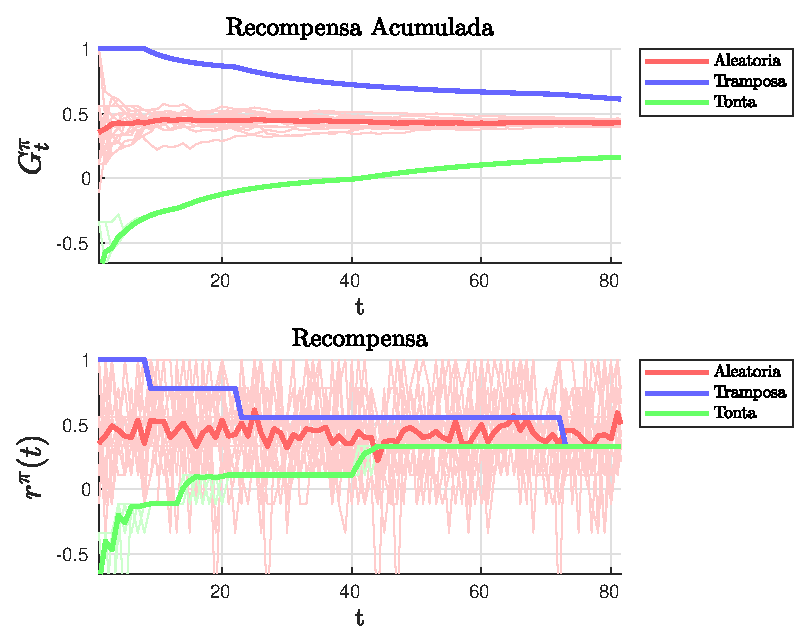
\includegraphics[scale=0.8]{img/policyref.eps}
    \caption{Políticas de referencias para un usuario concreto.}{Dado el caráter estocástico de las políticas, se dibuja la media de 20 experimentos.}
    \label{polref}
\end{figure}

\subsection{Caso 1: Usuario sin historial previo}

\subsection{Caso 2: Usuario con historial previo}

\chapter{Conclusiones} %
\bibliographystyle{apalike}
\bibliography{Thesbib}

\end{document}
 